\chapter{Backpropagation}\label{chapter:backpropagation}

\reviewcomment{Text will be revised and figures updated. Some figures missing.}

\newcommand{\xin}{\mathbf{x}_{\texttt{in}}}
\newcommand{\xout}{\mathbf{x}_{\texttt{out}}}

A key idea of neural nets is to decompose computation into a series of modular blocks. Each block takes in an input and produces an output: 

\begin{figure}[h]
    \centering
    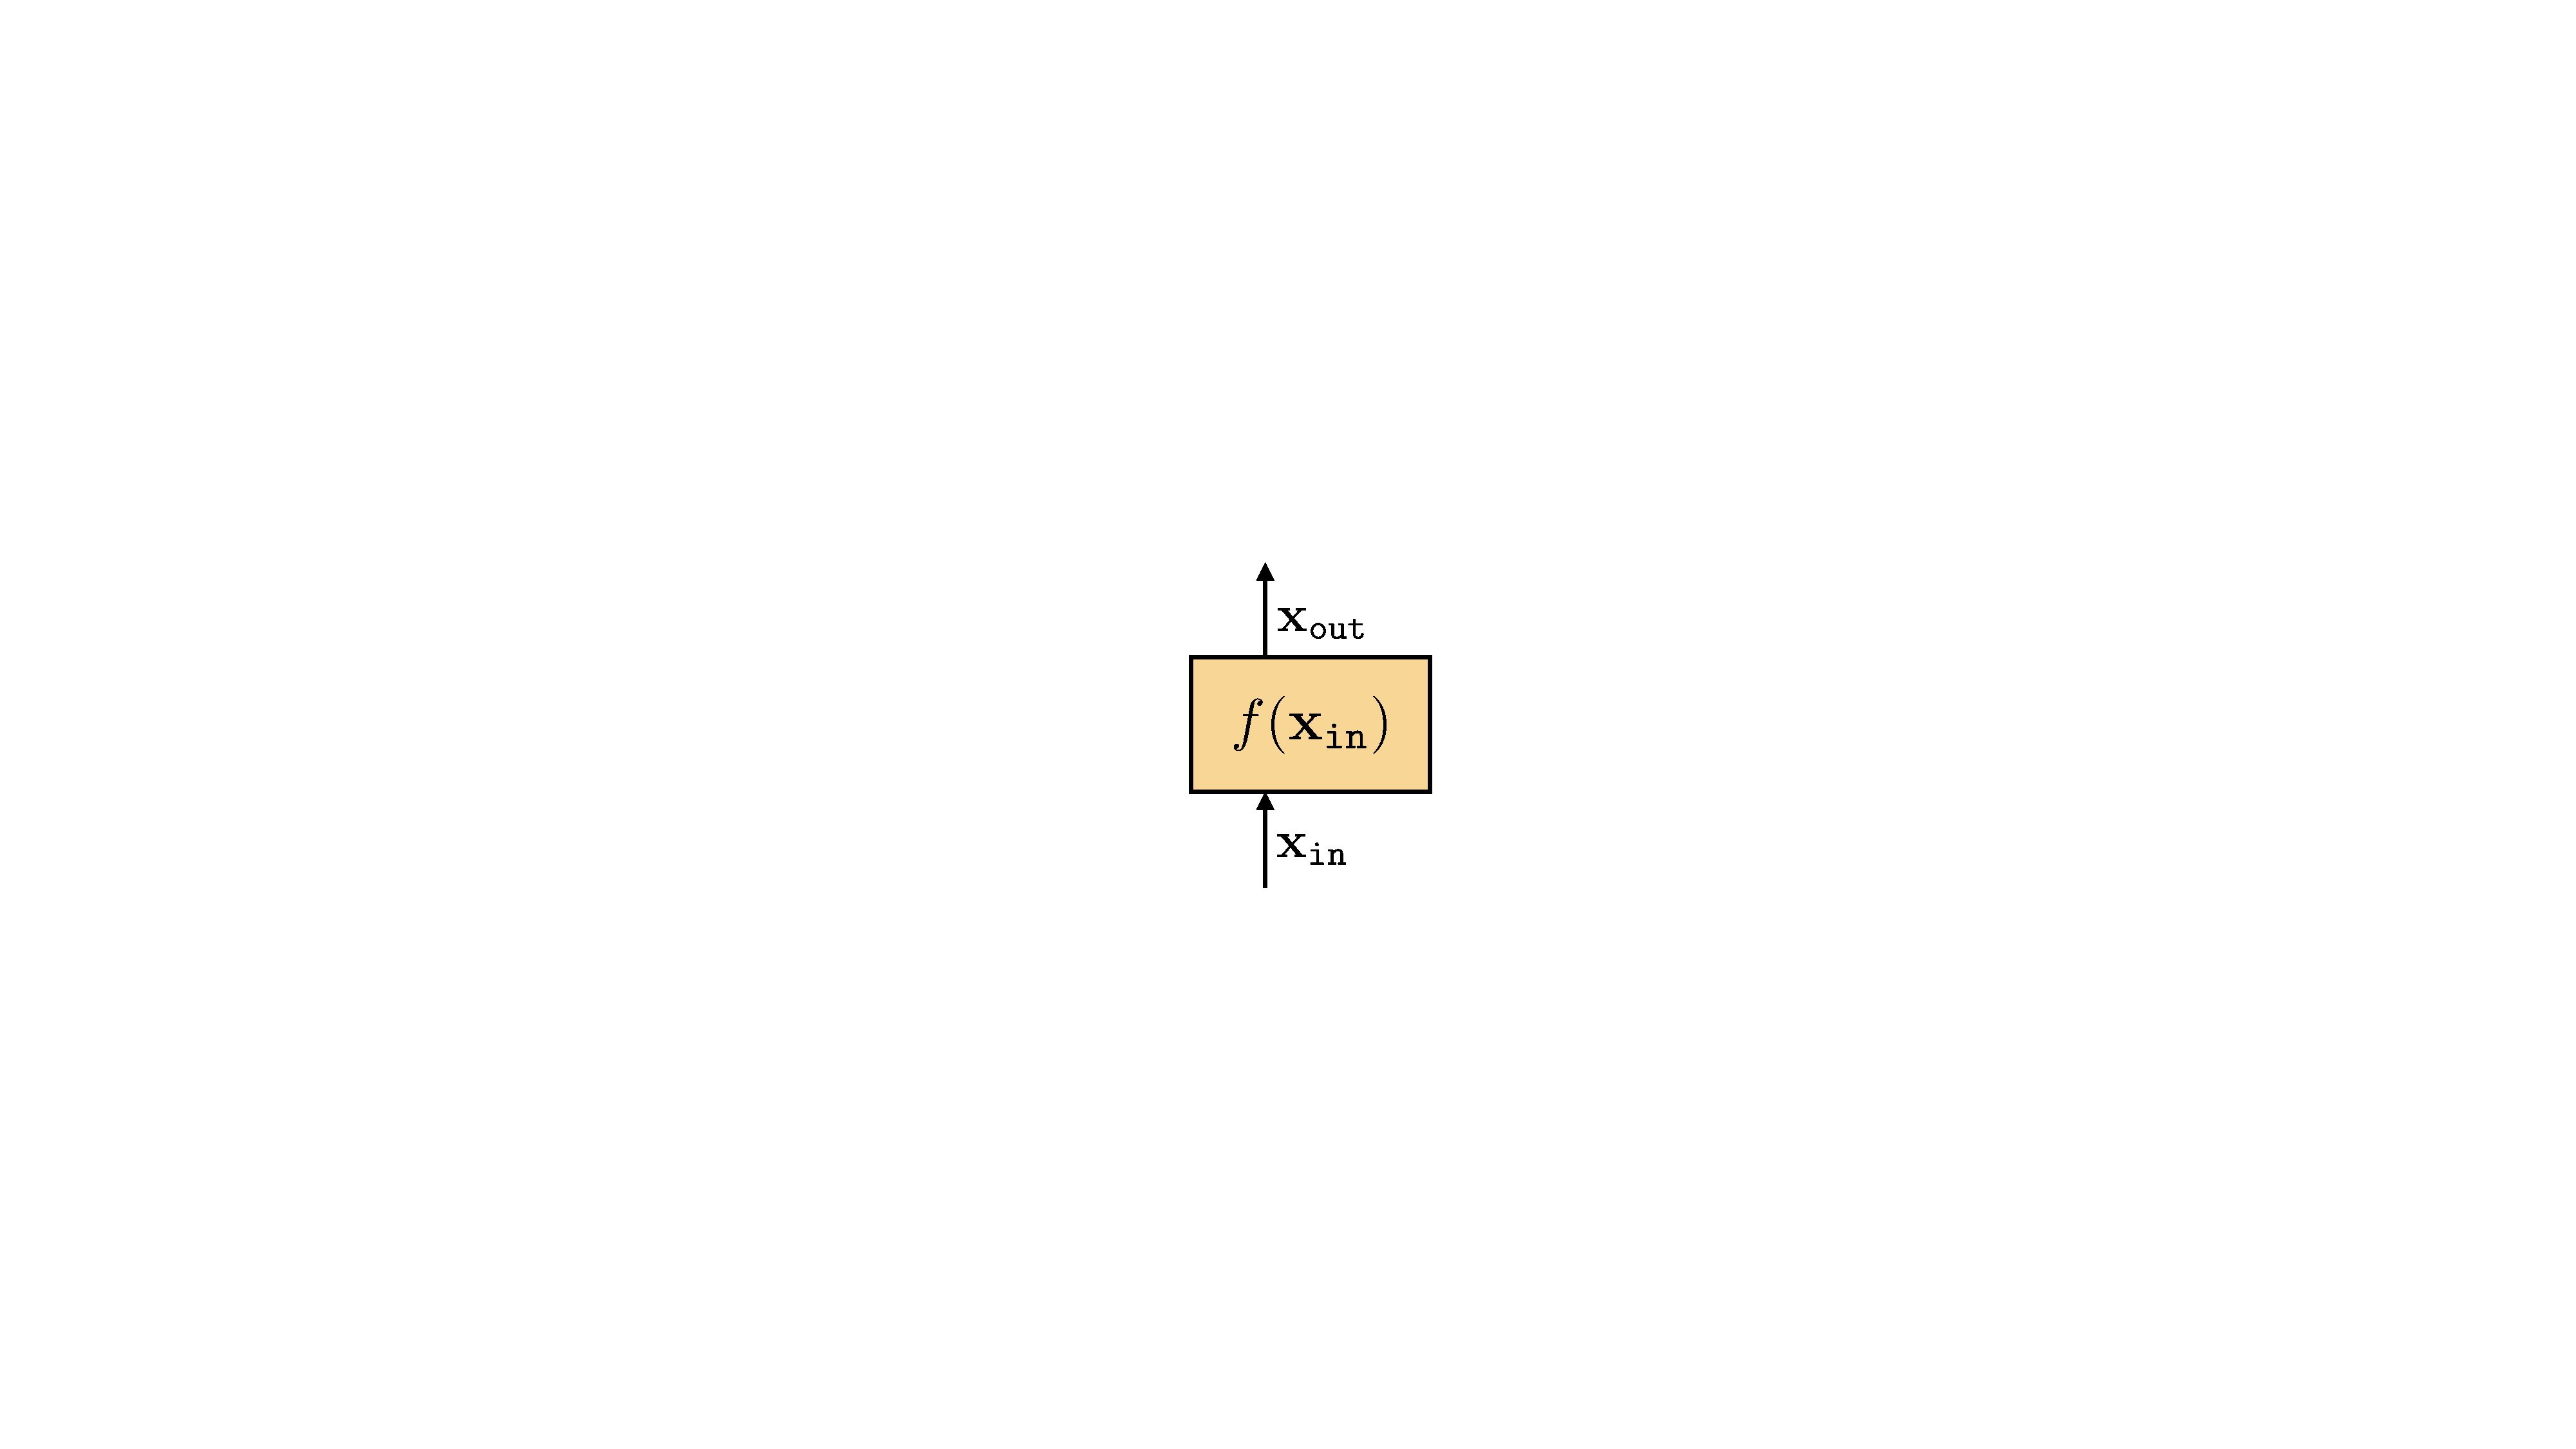
\includegraphics[width=0.18\linewidth]{./figures/backpropagation/mod_block.pdf}
    \label{fig:mod_block}
\end{figure}

In general, the building blocks are differentiable, so we can compute the gradient $\frac{\partial \xout}{\partial \xin}$. In the general case, $f$ takes in multiple inputs and spits out multiple outputs, so $\xin$ and $\xout$ are vectors and $\frac{\partial \xout}{\partial \xin}$ is a Jacobian matrix.%of the output, $\xout$, as some function, $g$, of the input, $\xin$ and the parameters of the block, $\theta$:
\marginnote{In some cases, the block might not be analytically differentiable, but we can estimate the gradient via sampling, e.g., using {\bf finite differences}:
\medbreak
    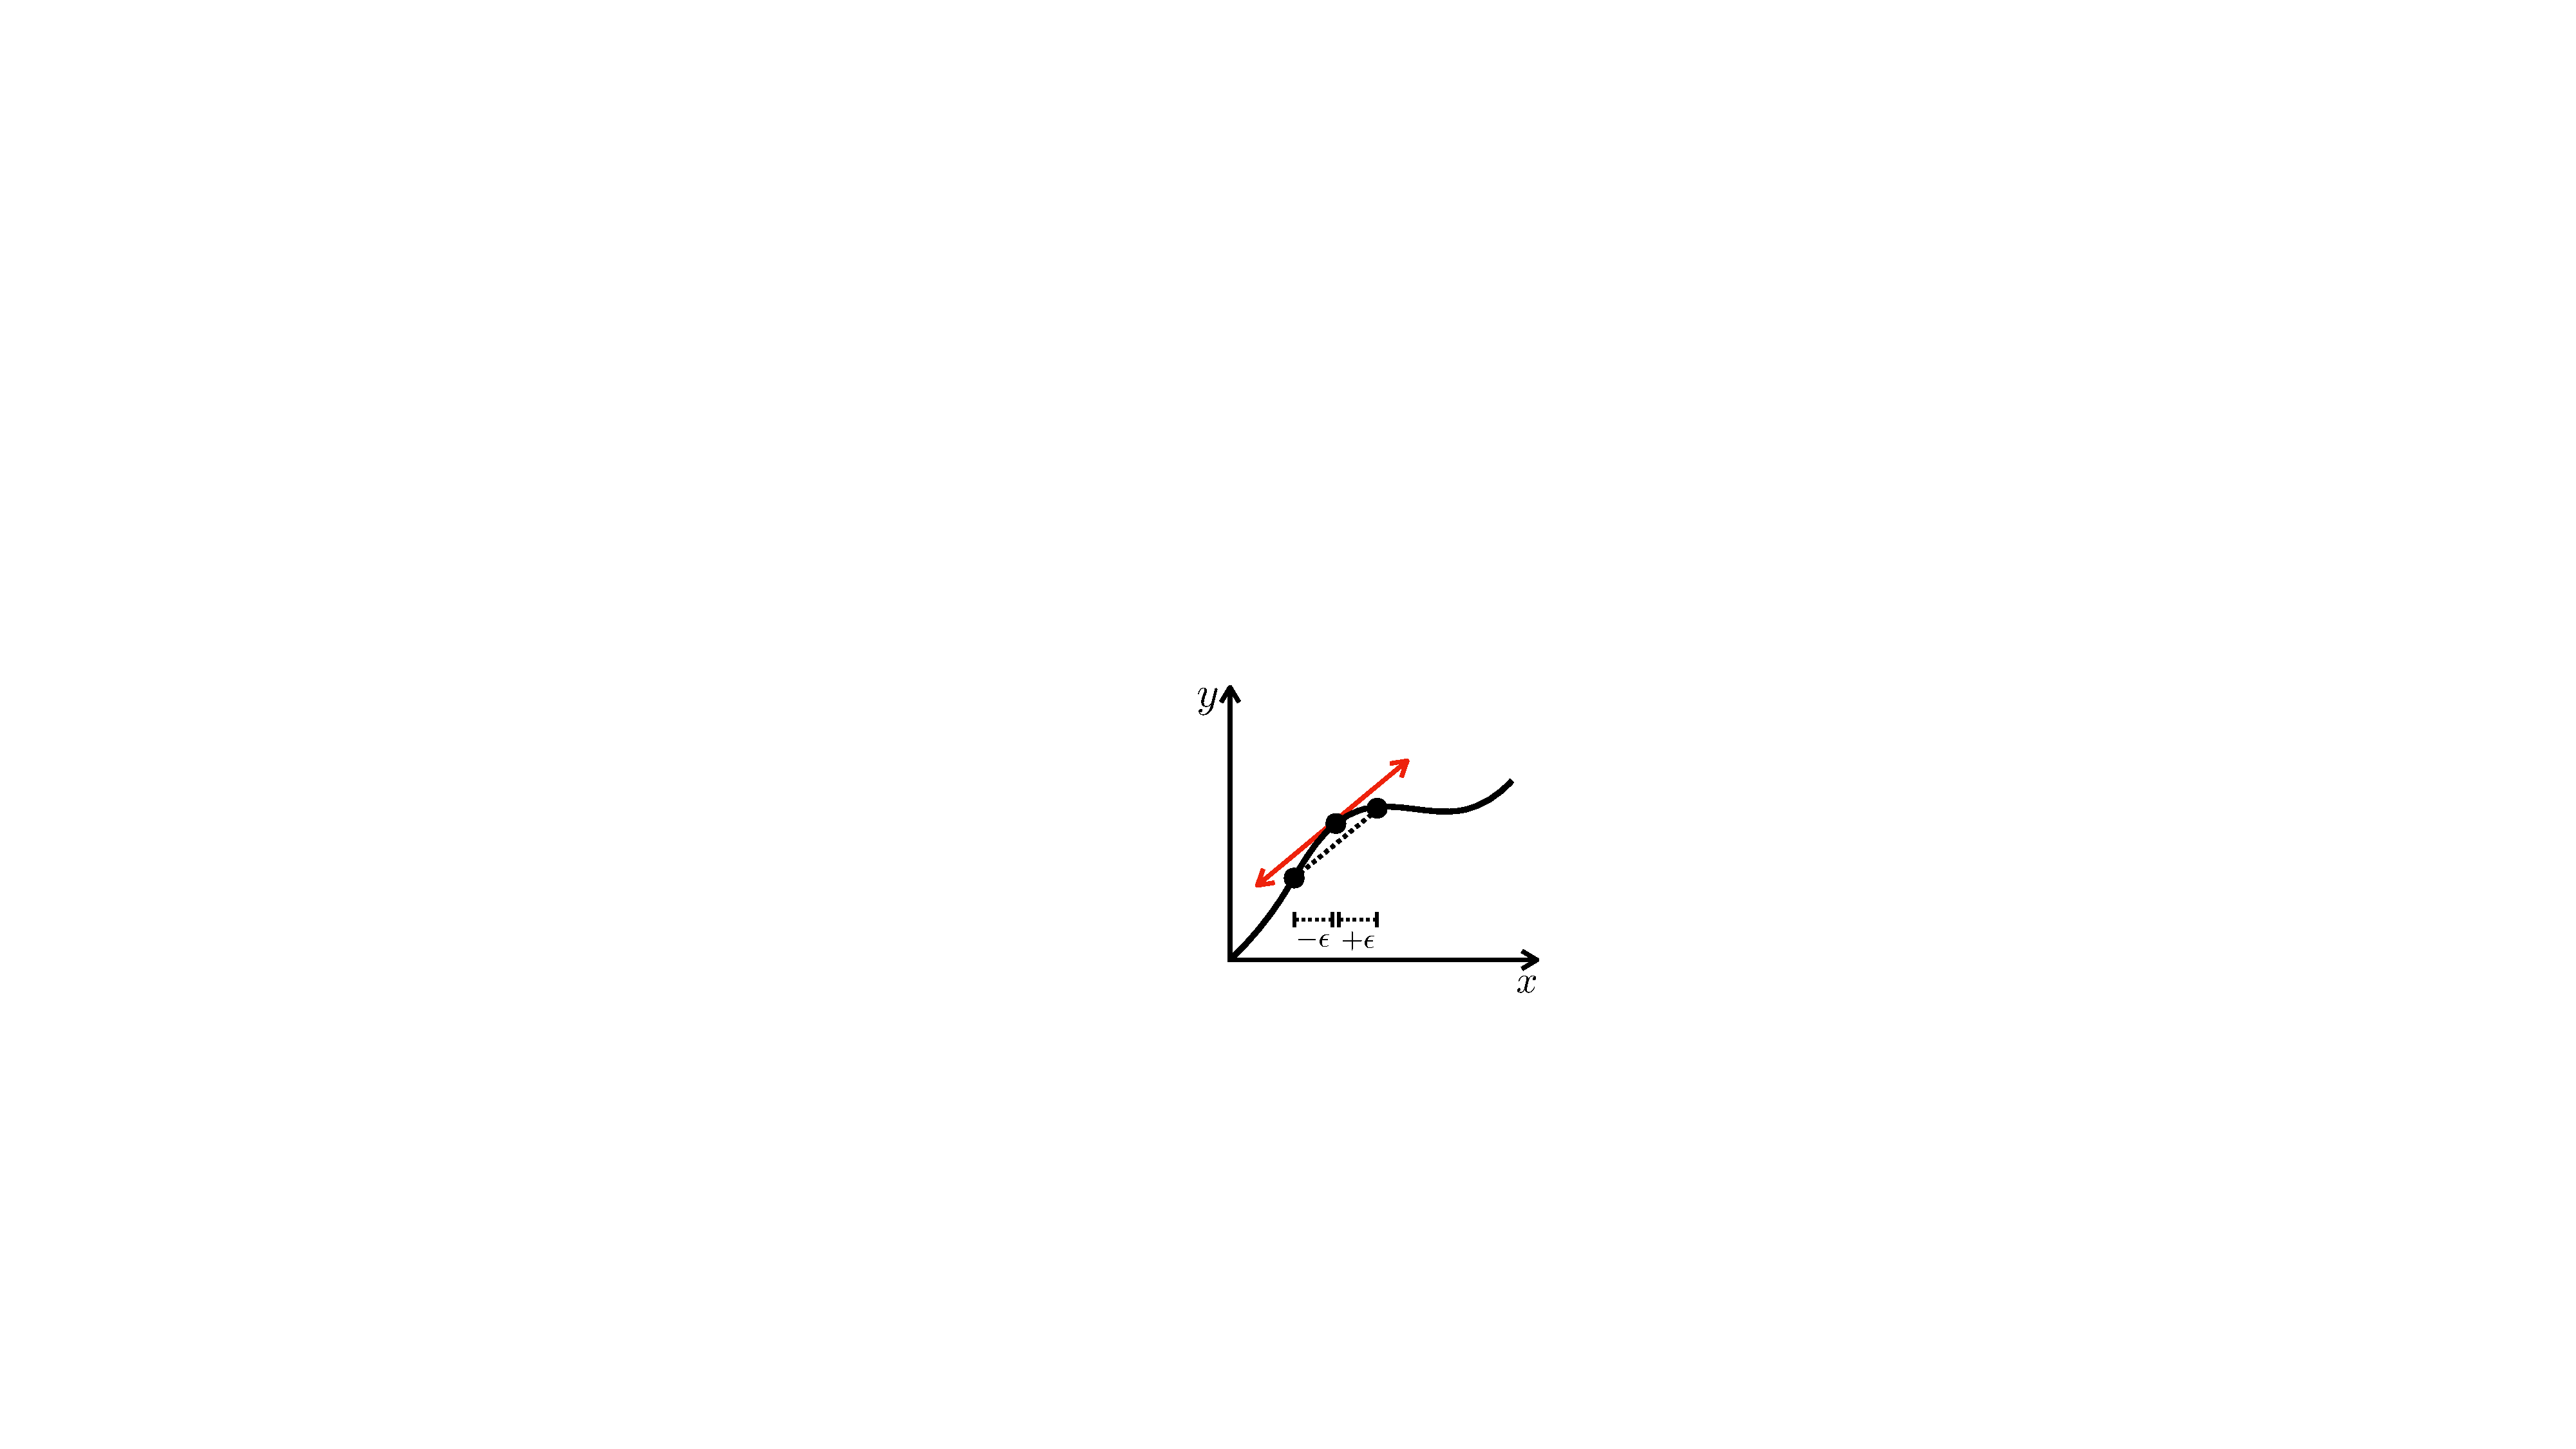
\includegraphics[width=0.8\linewidth]{./figures/backpropagation/finite_diffs.pdf}
}[-0.2cm]
%\begin{align}
%    \frac{\partial \xout}{\partial \xin} = g(\xin, \theta)
%\end{align}

When blocks are composed, we can compute the gradient of the total network using the chain rule from calculus:\\
\\
%\begin{SCfigure}[h]
  \hspace*{0.10\linewidth}\begin{minipage}{.10\textwidth}
    \centering
    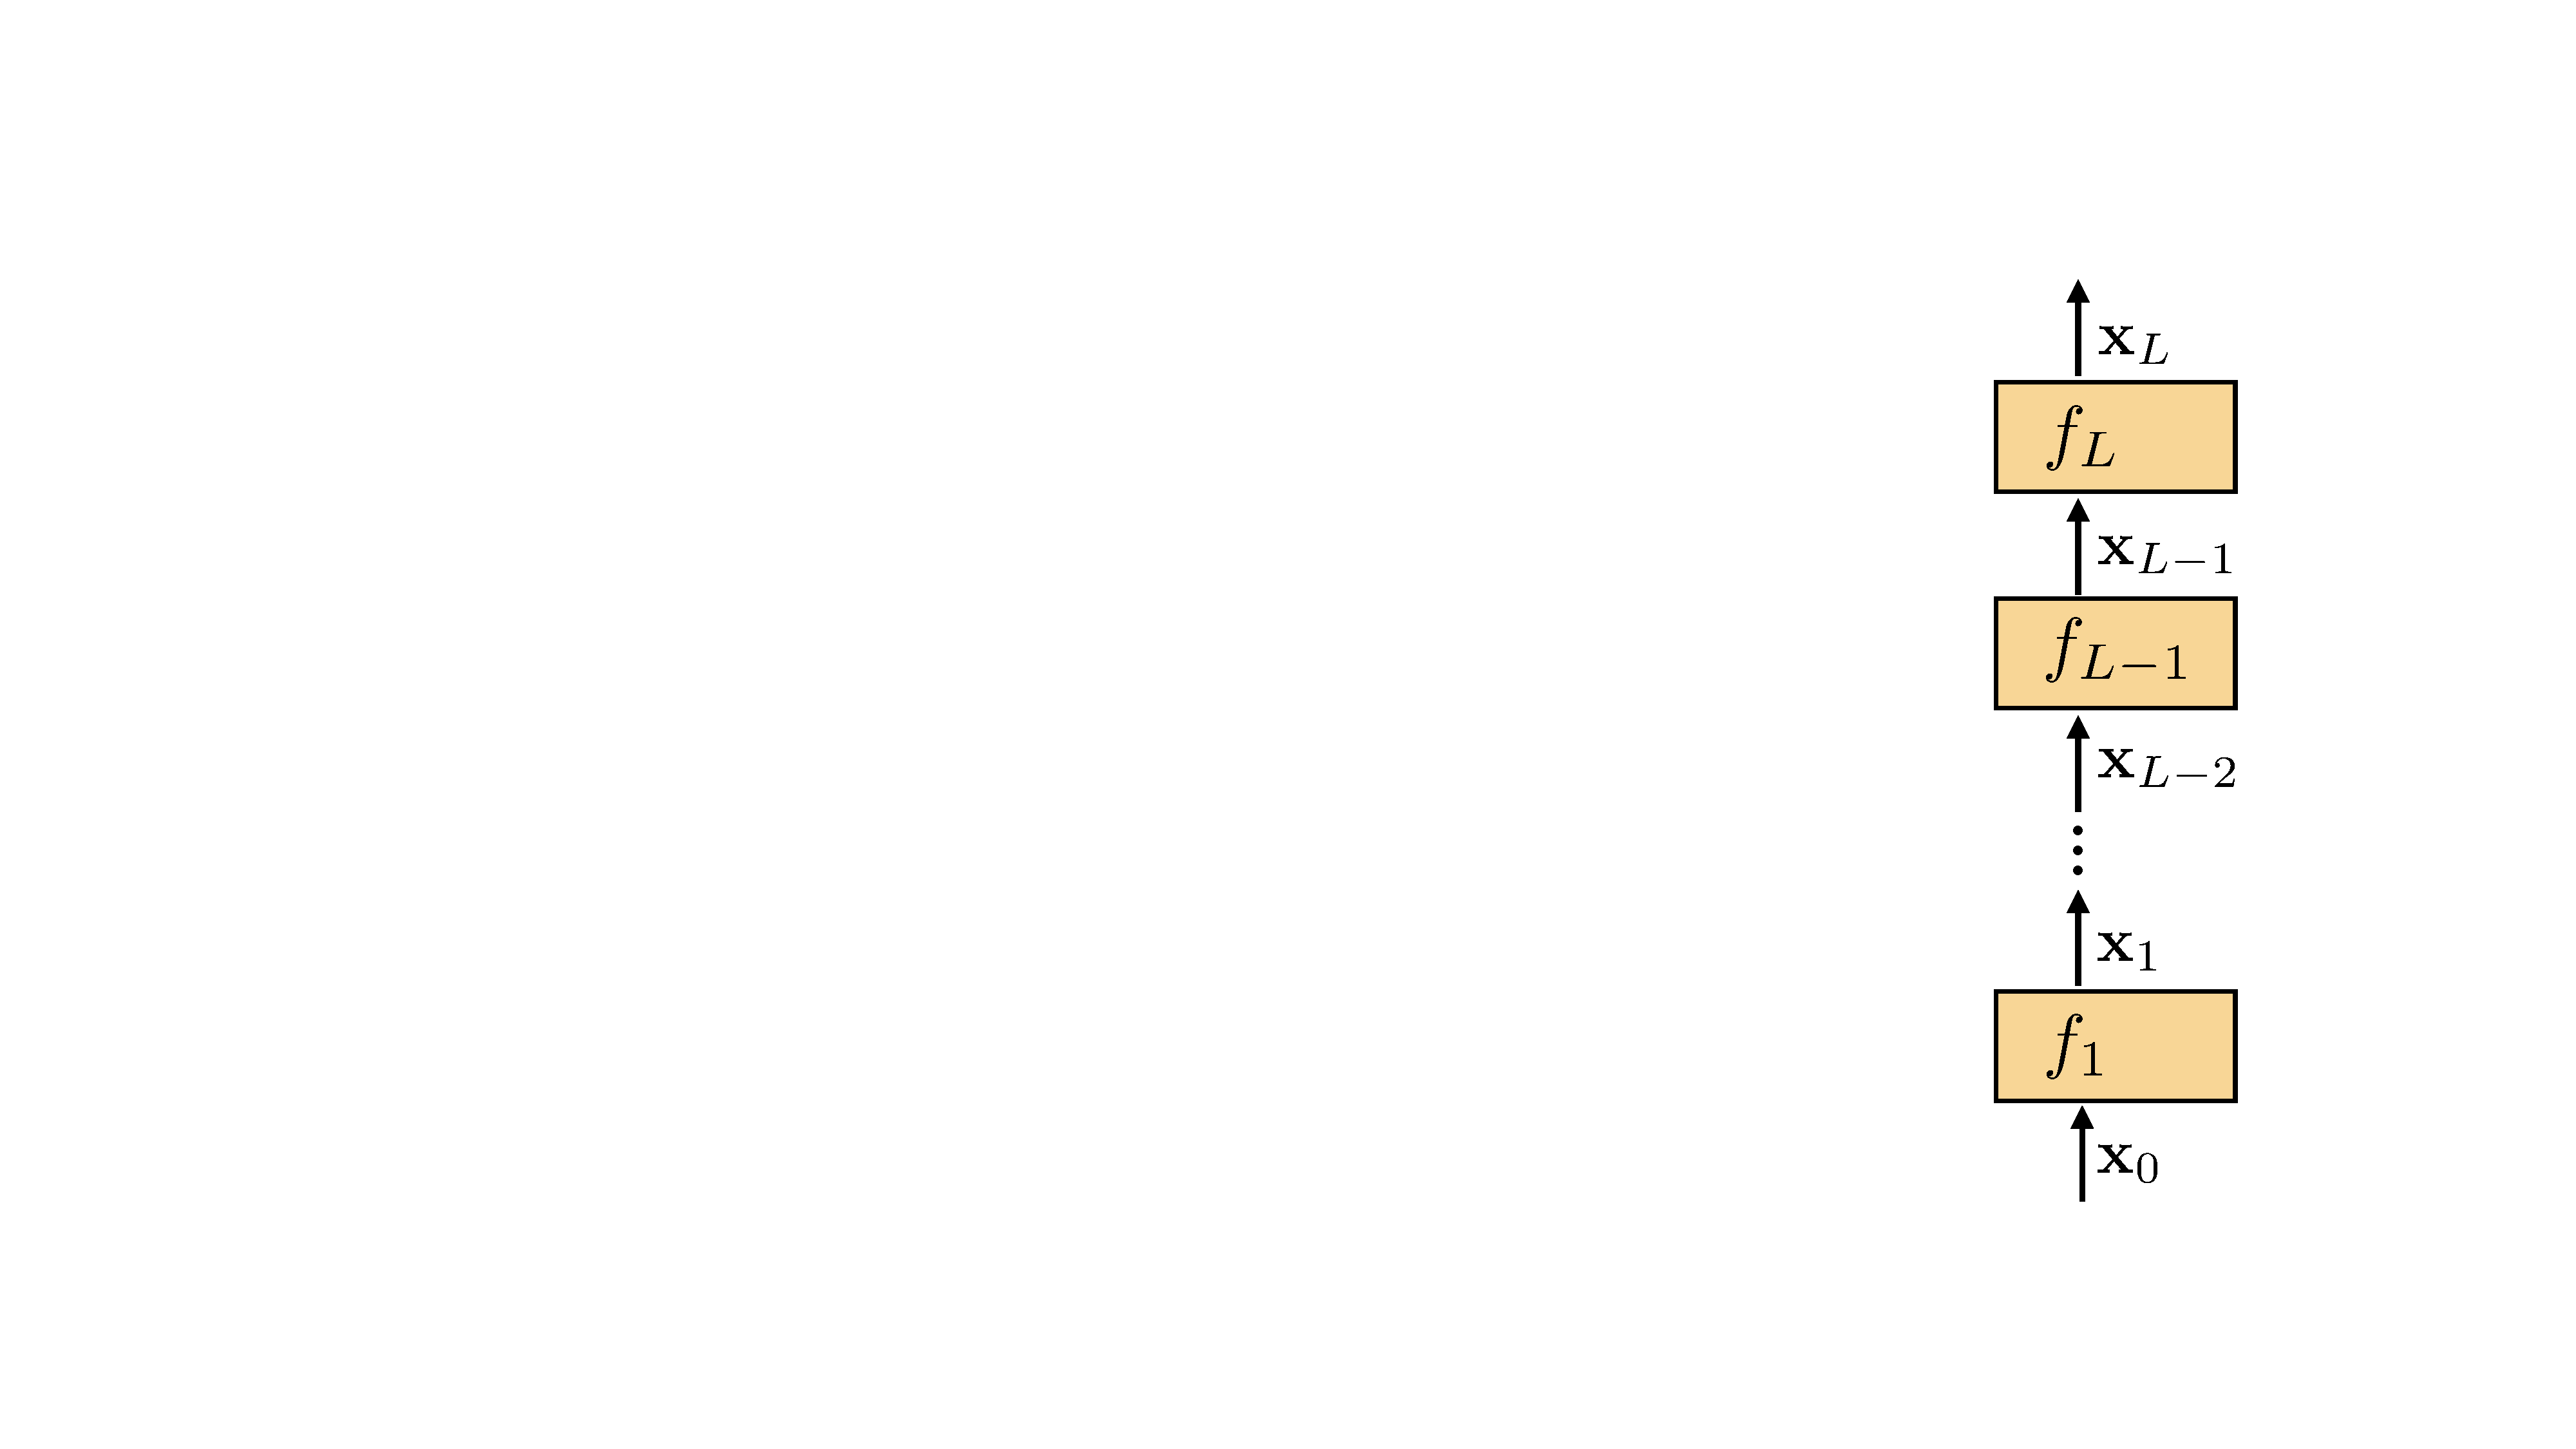
\includegraphics[width=1.0\linewidth]{./figures/backpropagation/composed_modules.pdf}
    \label{backpropagation:composed_modules}
  \end{minipage}
  \begin{minipage}{0.80\textwidth}
    \begin{align}
        \frac{\partial \mathbf{x}_{L}}{\partial \mathbf{x}_{1}} &= \frac{\partial \mathbf{x}_{L}}{\partial \mathbf{x}_{L-1}}\frac{\partial \mathbf{x}_{L-1}}{\partial \mathbf{x}_{L-2}} \cdots \frac{\partial \mathbf{x}_{1}}{\partial \mathbf{x}_{0}}\label{backprop:chain_rule}%\\
        %    &= \nabla_{\mathbf{x}} f^{L} \nabla_{\mathbf{x}} f^{L-1} \cdots \nabla_{\mathbf{x}} f^{1}
    \end{align}
    %\begin{align}
    %    \nabla_{\mathbf{x}} f^{l} &\equiv \frac{\partial f^{l}(\mathbf{x}^{l-1})}{\partial \mathbf{x}^{l-1}} \equiv \frac{\partial \mathbf{x}^{l}}{\partial \mathbf{x}^{l-1}}
    %\end{align}
  \end{minipage}
%\end{SCfigure}

{\bf Backpropagation} is an efficient algorithm for computing all the gradients in a network, i.e. $\frac{\partial \mathcal{L}}{\partial \theta_{l_i}}$ and $\frac{\partial \mathcal{L}}{\partial x_{l_i}}$ for all parameters $\theta_{l_i}$ and all {\bf neural activations} $x_{l_i}$. These gradients tell us how wiggling each individual parameter (or wiggling each individual activation) changes the loss $\mathcal{L}$. Clearly this is what we need if we want to adjust weights (or activations) to minimize the loss. We will also call the activations the \emph{inputs}, in this context, since we think of each layer of activations as the input data to the next layer of processing.\marginnote{``Neural activations" refers to the values neurons take on as they process data. We use this term for all the nodes in a network, regardless of whether they come after an activation function like \texttt{relu} or are any other node in the network.}[-1.8cm]


\section{The trick of backprop: reuse of computation}
Suppose we want to compute the gradients of the outputs on layers $L$ and $L+1$ with respect to the inputs $\mathbf{x}_0$. Following equation \ref{backprop:chain_rule} we have:

\begin{align}
    \frac{\partial \mathbf{x}_{L}}{\partial \mathbf{x}_{0}} =  \color{blue} \frac{\partial \mathbf{x}_{L}}{\partial \mathbf{x}_{L-1}}\frac{\partial \mathbf{x}_{L-1}}{\partial \mathbf{x}_{L-2}} \cdots \frac{\partial \mathbf{x}_{1}}{\partial \mathbf{x}_{0}}\\
    \frac{\partial \mathbf{x}_{L+1}}{\partial \mathbf{x}_{0}} = \frac{\partial \mathbf{x}_{L+1}}{\partial \mathbf{x}_{L}} \color{blue} \frac{\partial \mathbf{x}_{L}}{\partial \mathbf{x}_{L-1}}\frac{\partial \mathbf{x}_{L-1}}{\partial \mathbf{x}_{L-2}} \cdots \frac{\partial \mathbf{x}_{1}}{\partial \mathbf{x}_{0}}
\end{align}
Rather than evaluating both equations separately, we notice that all the blue terms are shared. Indeed, once we've computed $\frac{\partial \mathbf{x}_{L}}{\partial \mathbf{x}_{0}}$, we can compute $\frac{\partial \mathbf{x}_{L+1}}{\partial \mathbf{x}_{0}}$ with just one more multiply:
\begin{align}
    \frac{\partial \mathbf{x}_{L+1}}{\partial \mathbf{x}_{0}} = \frac{\partial \mathbf{x}_{L+1}}{\partial \mathbf{x}_{L}} \frac{\partial \mathbf{x}_{L}}{\partial \mathbf{x}_{0}}
\end{align}
This is the whole trick of backpropagation: rather than computing each layer's gradients independently, observe that they share many of the same terms, so we might as well calculate each shared term once and reuse them. \marginnote{This strategy, in general, is called {\bf dynamic programming}.}[-0.6cm]

In general, we can compute the gradient of any layer of outputs, $i$, with respect to any layer of inputs, $j$ as:
\begin{align}
    \frac{\partial \mathbf{x}_{i}}{\partial \mathbf{x}_{j}} = \frac{\partial \mathbf{x}_{i}}{\partial \mathbf{x}_{i-1}} \frac{\partial \mathbf{x}_{i-1}}{\partial \mathbf{x}_{j}}\label{eqn:backprop:trick}
\end{align}
The trick, again, is that if we have already computed $\frac{\partial \mathbf{x}_{i-1}}{\partial \mathbf{x}_{j}}$, computing $\frac{\partial \mathbf{x}_{i}}{\partial \mathbf{x}_{j}}$ is easy.

%Mathematically, computing the gradients of a composition of differentiable blocks is quite easy. Suppose we are interested in the gradient of the loss with respect to the parameters on layer 2 of the network, $\theta^2$. 

\section{Loss as just another layer}
The outputs of a neural net, $\mathbf{x}_{L}$, are typically fed to a loss function $\mathcal{L}$, and it's the gradients of this loss that we care about for learning. To get the gradient $\frac{\partial \mathcal{L}}{\partial \mathbf{x}_{j}}$, we can simply think of the loss as one more layer of processing, which outputs a scalar $x_{L+1} = \mathcal{L}(\mathbf{x}_L)$. Then, using the same logic as in Eqn.~\ref{eqn:backprop:trick}, we can observe that:
\begin{align}
    \frac{\partial \mathcal{L}}{\partial \mathbf{x}_{j}} = \frac{\partial \mathcal{L}}{\partial \mathbf{x}_{L}} \frac{\partial \mathbf{x}_{L}}{\partial \mathbf{x}_{j}}\label{eqn:backprop:backprop_through_loss}
\end{align}
%The idea here is that the loss $\mathcal{L}$ is just one more layer of processing, so we have just defined the final layer as $\mathbf{x}_{L} = \mathcal{L}$ and then applied Eqn.~\ref{eqn:backprop:trick}.

\section{Gradients with respect to the network parameters}
So far we have only considered computing gradients with respect to activations. But for learning, what we really care about is the gradient of the loss with respect to the parameters, i.e. $\frac{\partial \mathcal{L}}{\partial \theta}$, since this will tell us how to update the parameters to minimize the loss. Fortunately, this is easy, given the tools above. The gradient of the loss with respect to the parameters on some layer $l$, are given by one more application of the chain rule:
\begin{align}
\frac{\partial \mathcal{L}}{\partial \theta_l} &= \frac{\partial \mathcal{L}}{\partial \mathbf{x}_{l}} \frac{\partial \mathbf{x}_{l}}{\partial \theta_l} \label{eqn:backprop:update_theta}
\end{align}
Remember that $\mathbf{x}_{l} = f_l(\mathbf{x}_{l-1}, \theta_l)$, so we can equivalently rewrite Eqn.~\ref{eqn:backprop:update_theta} as:
\begin{align}
\frac{\partial \mathcal{L}}{\partial \theta_l} &= \frac{\partial \mathcal{L}}{\partial \mathbf{x}_l} \frac{\partial f_l(\mathbf{x}_{l-1}, \theta_l)}{\partial \theta_l}
\end{align}

\section{Forward and backward pass for a single layer}
The above derivations show us that the gradient of the loss with respect to each layer $l$'s activations and parameters, $\frac{\partial \mathcal{L}}{\partial \mathbf{x}_{l}}$ and $\frac{\partial \mathcal{L}}{\partial \theta_l}$, can be computed \emph{locally}, given just the definition of the layer (i.e. the function $f$ and its gradients $\frac{\partial f_l}{\partial \mathbf{x}_l}$ and $\frac{\partial f_l}{\partial \theta_l}$), and two inputs: activations propagated \emph{forward} from the previous layer, $\mathbf{x}_{l-1}$, and gradients propagated \emph{backwards} from the subsequent layer, $\frac{\partial \mathcal{L}}{\partial \mathbf{x}_{l}}$. Each module's local computations look like this:
%So, backprop exploits the property that each subsequent module's gradients are a simple function of the previous module's gradient. In backprop, each module looks like this:
\begin{figure}[h]
    \centering
    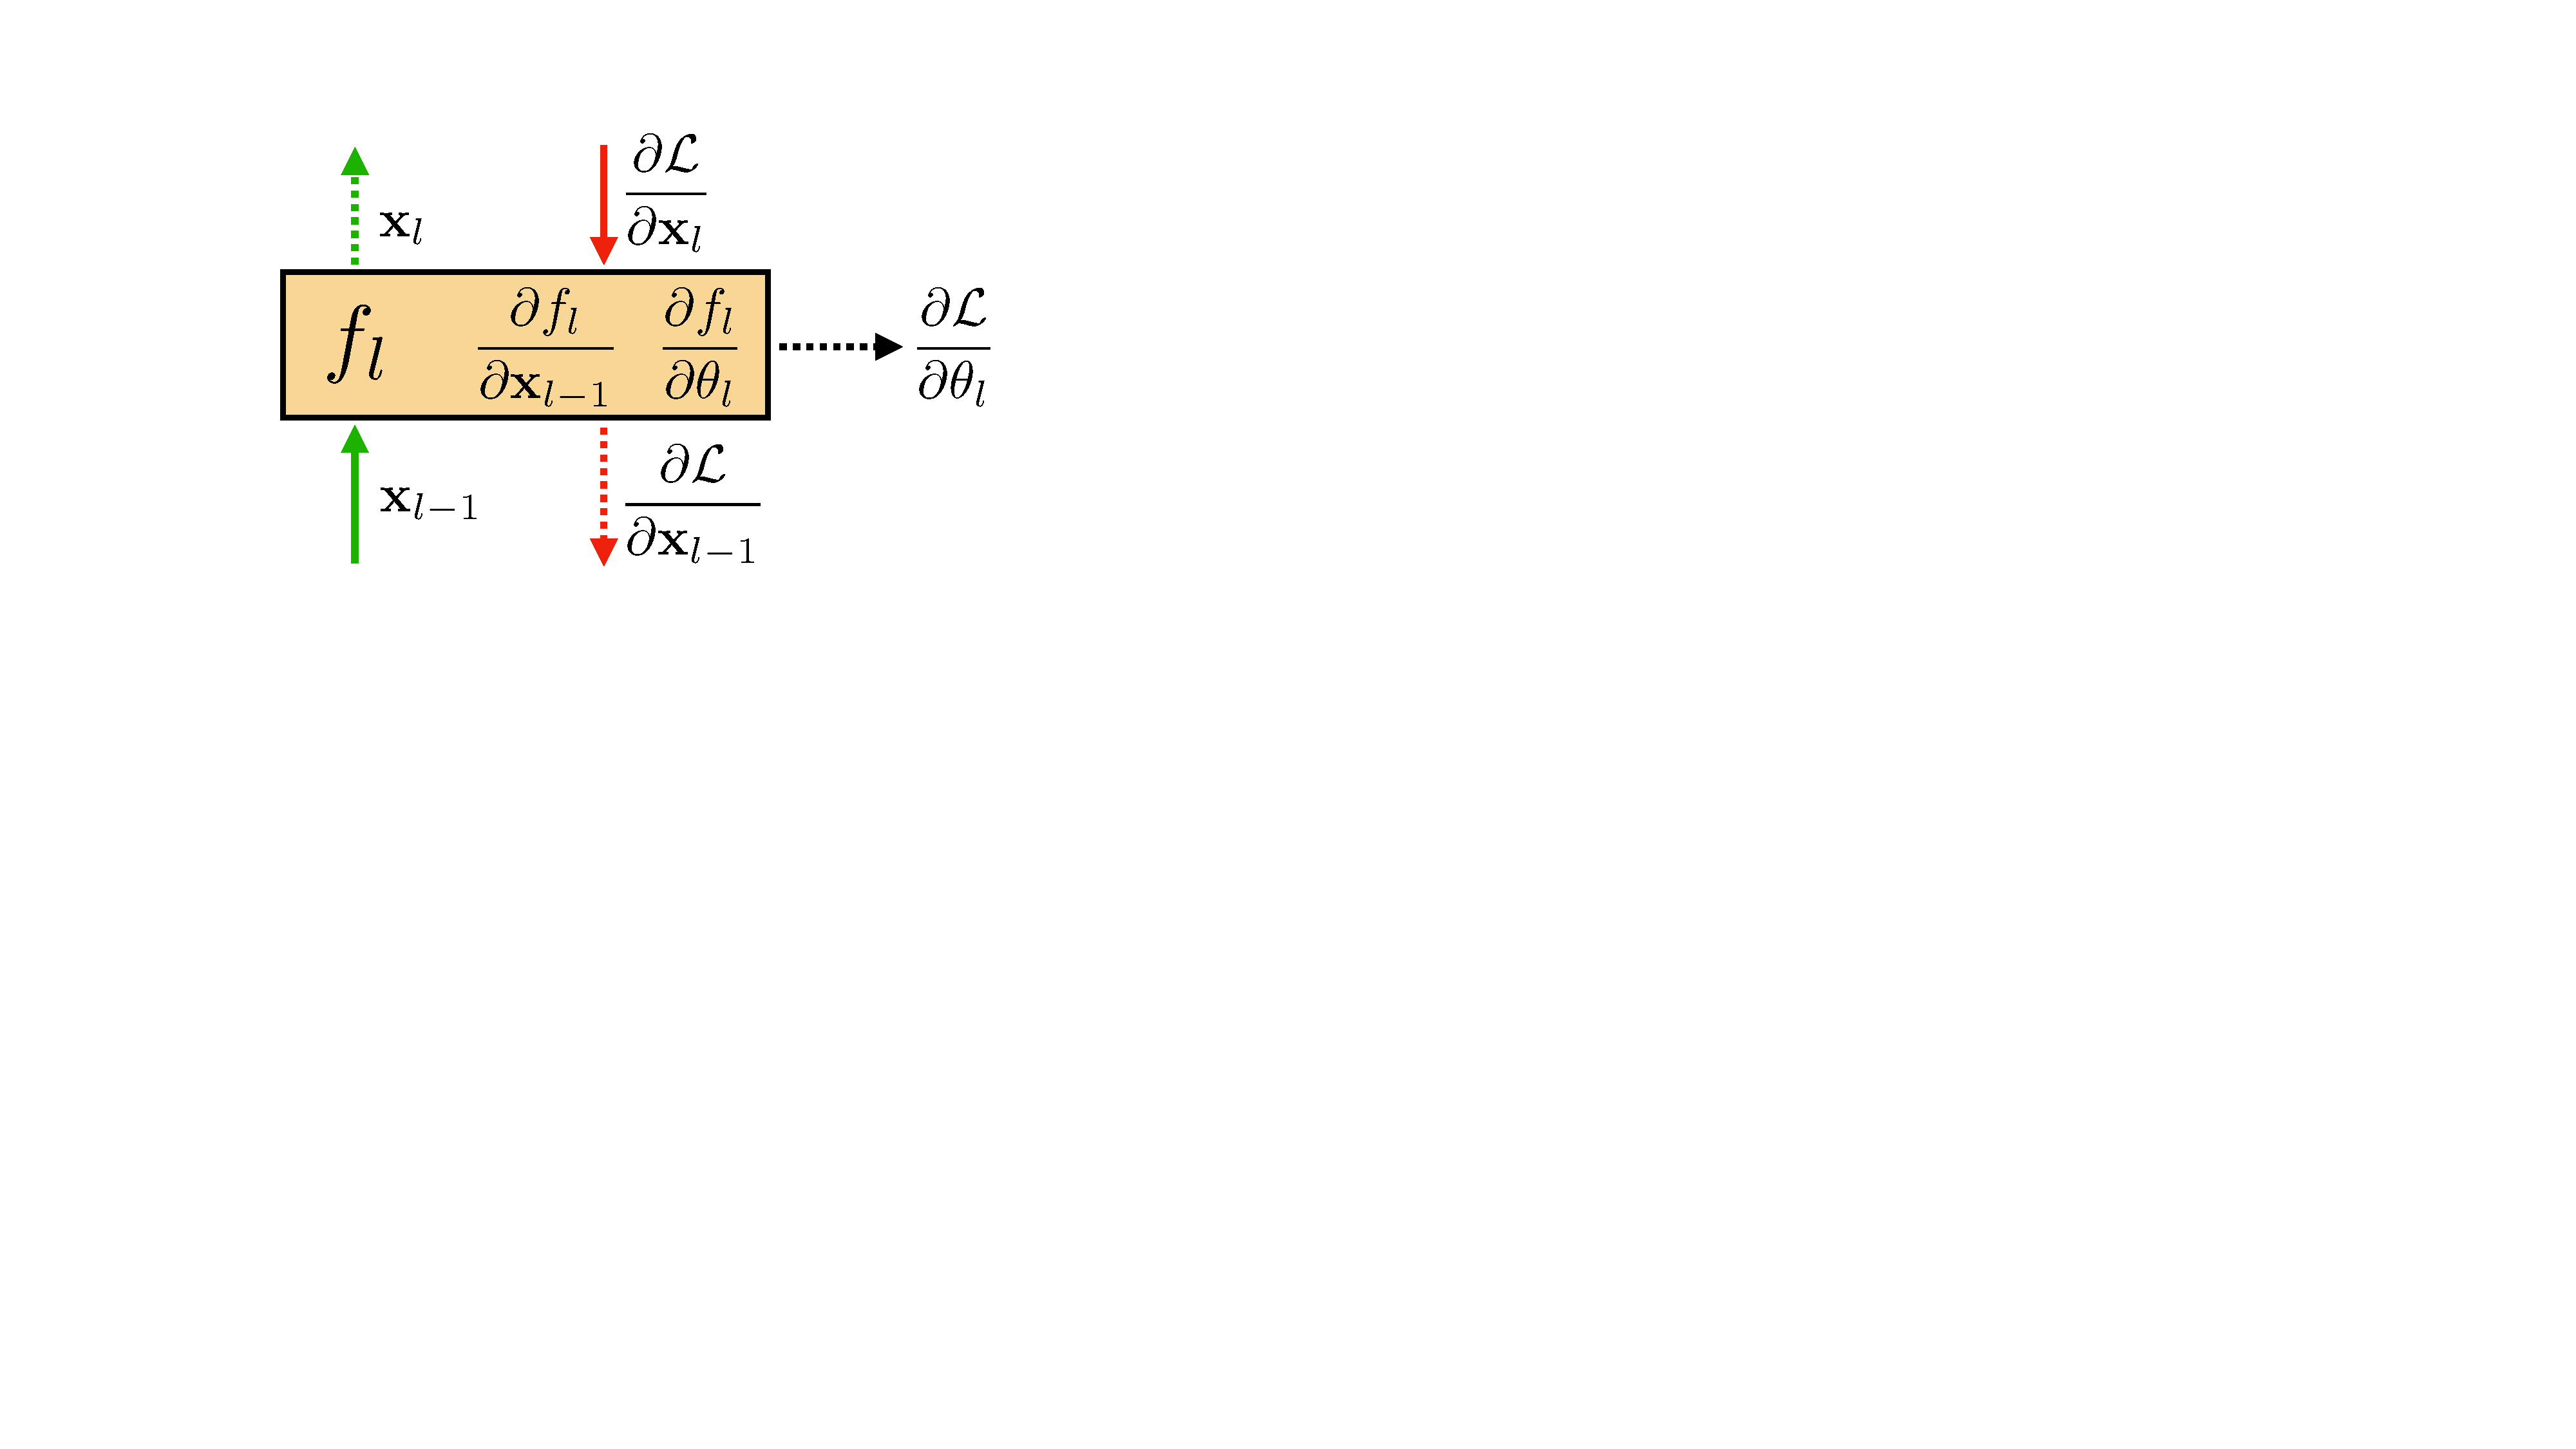
\includegraphics[width=0.5\linewidth]{./figures/backpropagation/backprop_mod_block.pdf}
    \label{fig:backprop_mod_block}
\end{figure}

The equations for the three outputs are:
\begin{align}
    \mathbf{x}_{l} &= f_l(\mathbf{x}_{l-1}, \theta_l) & \quad\quad \triangleleft \quad \text{foward propagation}\\
    \frac{\partial \mathcal{L}}{\partial \mathbf{x}_{l-1}} &= \frac{\partial \mathcal{L}}{\partial \mathbf{x}_{l}} \frac{\partial f_l}{\partial \mathbf{x}_{l-1}} & \quad\quad \triangleleft \quad \text{backward propagation} \label{update_x}\\
    \frac{\partial \mathcal{L}}{\partial \theta_l} &= \frac{\partial \mathcal{L}}{\partial \mathbf{x}_{l}} \frac{\partial f_l}{\partial \theta_l} & \quad\quad \triangleleft \quad \text{parameter gradient} \label{update_theta}
\end{align}
%\begin{align}
%    \xout &= f^l(\xin)\\
%    \frac{\partial \mathcal{L}}{\partial \mathbf{x}^l}\bigg|_{\xin} &= \frac{\partial \mathcal{L}}{\partial \mathbf{x}^l}\bigg|_{\xout} \frac{\partial f}{\partial \mathbf{x}^{(l-1)}}\bigg|_{\xin}\\
%    \frac{\partial \mathcal{L}}{\partial \theta^l}\bigg|_{\xin} &= \frac{\partial \mathcal{L}}{\partial \mathbf{x}^l}\bigg|_{\xout} \frac{\partial f}{\partial \theta^{(l-1)}}\bigg|_{\theta}
%\end{align}
%These equations are just the chain rule, which might be more obvious by plugging in $\frac{\partial f_l}{\partial \mathbf{x}_l} \equiv \frac{\partial \mathbf{x}_{l+1}}{\partial \mathbf{x}_l}$ and $\frac{\partial f_l}{\partial \theta_l} \equiv \frac{\partial \mathbf{x}_{l+1}}{\partial \theta_l}$.

\section{Forward and backward pass through multiple layers}
To compute all the gradients in this local manner, we need to order the operations so that $\mathbf{x}_l$ and $\frac{\partial \mathcal{L}}{\partial \mathbf{x}_{l}}$ are available before computing the gradients for layer $l$. The way to do this is run a complete {\bf forward pass} through the network, computing $\mathbf{x}_2$, then $\mathbf{x}_3$, and so forth, then run a complete {\bf backward pass} through the network, computing $\frac{\partial \mathcal{L}}{\partial \mathbf{x}_{L}}$ and $\frac{\partial \mathcal{L}}{\partial \theta_{L}}$, then $\frac{\partial \mathcal{L}}{\partial \mathbf{x}_{L-1}}$ and $\frac{\partial \mathcal{L}}{\partial \theta_{L-1}}$ and so forth. 

\newpage
A complete forward pass followed by a complete backward pass corresponds to following the green arrows and then the red arrows through the following computation graph:
\begin{figure}[h!]
    \centering
    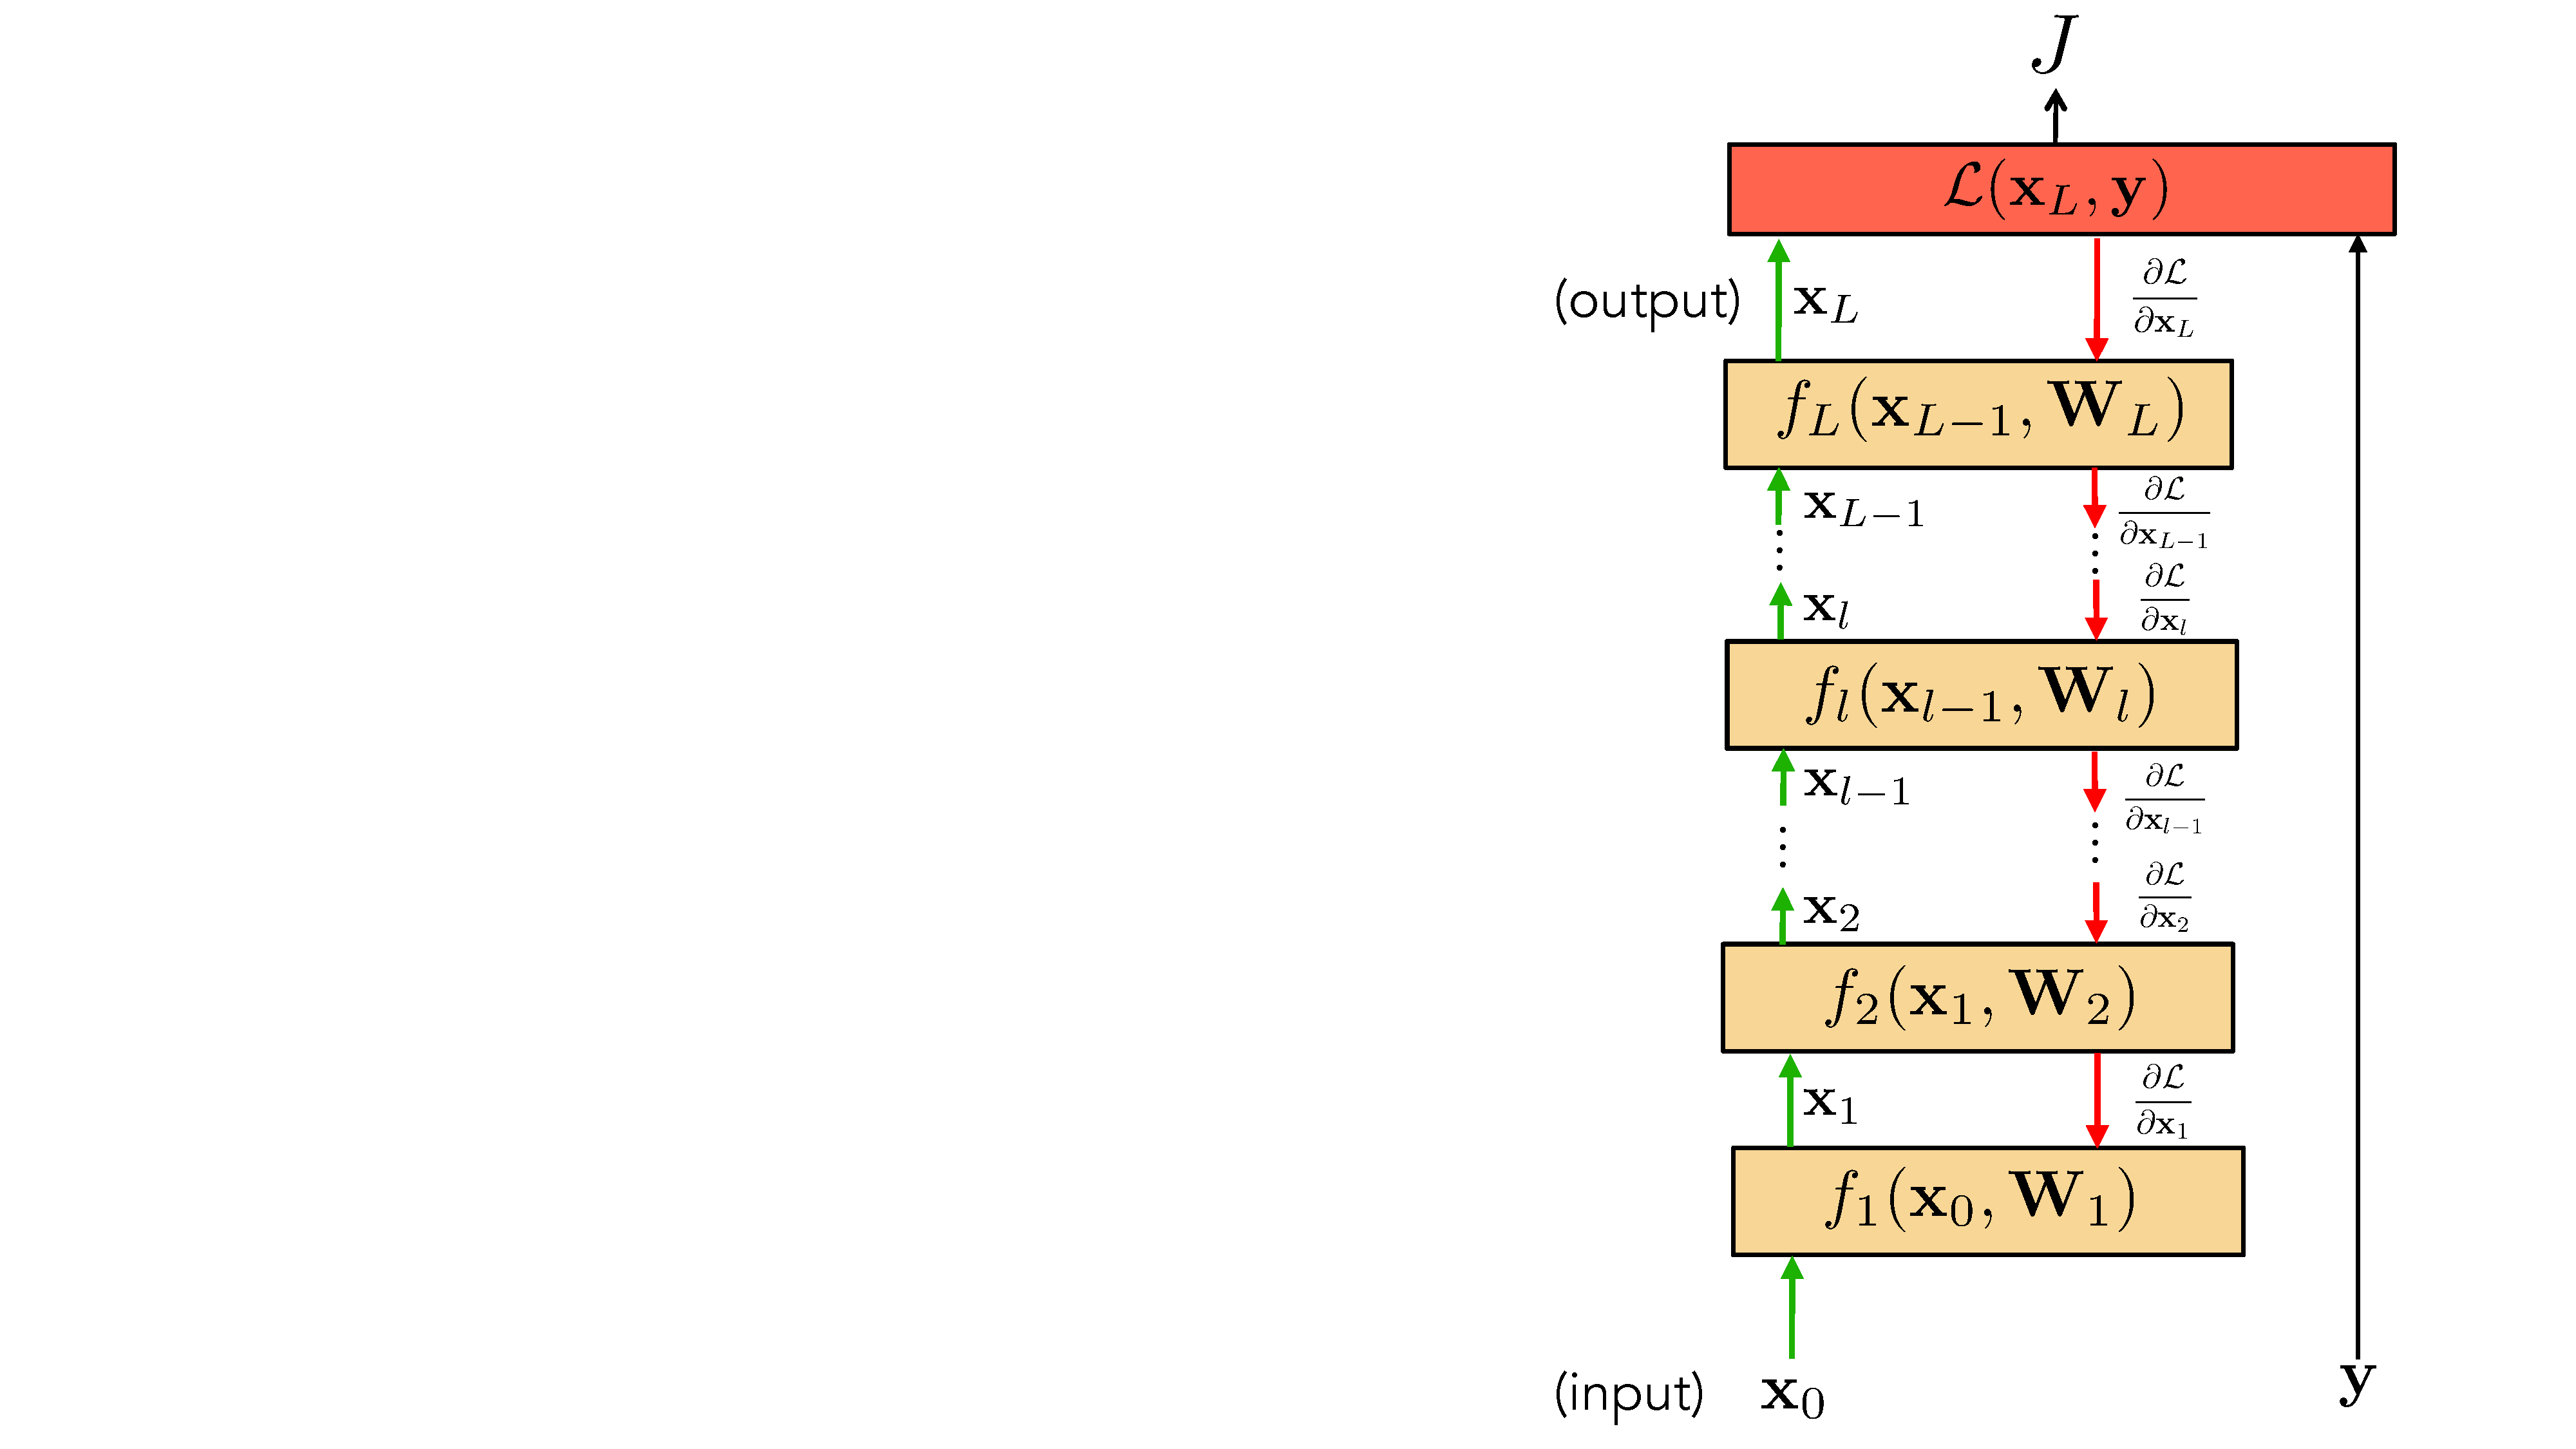
\includegraphics[width=0.45\linewidth]{./figures/backpropagation/backprop_through_multiple_layers.pdf}
    \label{fig:backprop_through_multiple_layers}
\end{figure}

%$f$ is known as the {\bf forward function} and $g$ is the {\bf backward function}. We also require a function, $h$ to compute the gradient of the loss with respect to the layer's parameters, $\frac{\partial \mathcal{L}}{\partial \theta}$.

%The gradients, with respect to either activations or parameters, can be computed as simple functions of just the terms in this diagram:
%\begin{align}
%    \xout &= f(\xin, \theta)\\
%    \frac{\partial \mathcal{L}}{\partial \xin} &= \frac{\partial \mathcal{L}}{\partial \xout} \frac{\partial \xout}{\partial \xin}\\
%    \frac{\partial \mathcal{L}}{\partial \theta} &= \frac{\partial \mathcal{L}}{\partial \xout} \frac{\partial \xout}{\partial \theta}
%\end{align}

%When we have multiple layers, each layer $l$'s inputs and outputs, in both the forward and backward directions, can be computed just with these three layer-specific equations, $f^l$, $g^l$, and $h^l$. It doesn't matter how deep the net is or how many modules there are. Once you know $\xin$ and $\frac{\partial \mathcal{L}}{\partial \xout}$, you can compute the output $\xout$ and the gradients $\frac{\partial \mathcal{L}}{\partial \xin}$ and $\frac{\partial \mathcal{L}}{\partial \theta}$ for the layer.

%Notice that you really only need to define one function $f^l$, which is the function the layer computes in the forward direction. $g^l$ and $h^l$ just depend on particular derivatives of $f^l$:% as well as the inputs to the layer (in the forward and backward directions):

%\begin{align}
%    g(\frac{\partial \mathcal{L}}{\partial \xout}, \theta, \xin) = \frac{\partial \mathcal{L}}{\partial \xout} \frac{\partial f^l}{\partial \xin}\\
%    h(\frac{\partial \mathcal{L}}{\partial \xout}, \theta, \xin) = \frac{\partial \mathcal{L}}{\partial \xout} \frac{\partial f^l}{\partial \theta}
%\end{align}

%where we have made use of $f^l(\xin) = \xout$.

%\begin{align}
%    g = \frac{\partial \mathcal{L}}{\partial \xout} \frac{\partial \xout}{\partial \xin}
%\end{align}

\section{Backprop to optimize total cost $J$}
Once we have computed a gradient with backprop, we can use it to optimize our neural network via gradient descent. First we will briefly review gradient descent, then we will plug in the gradient from backprop.

\begin{algorithm}[h]
\label{gradient_descent}
\SetAlgoVlined
\DontPrintSemicolon
\caption{Gradient descent}
{\bf Input:} initial parameter vector $\theta^{0}$, data $\{\mathbf{x}^{(i)},\mathbf{y}^{(i)}\}_{i=1}^N$, learning rate $\eta$\;
{\bf Output:} trained model $f_{\theta^{N}}$\;
\For{\upshape $k= 1, \dots, K$}{
    $J = \sum_{i=1}^N \mathcal{L}(f_{\theta^{k-1}}(\mathbf{x}^{(i)}),\mathbf{y}^{(i)})$\;
    $\theta^{k} \leftarrow \theta^{k-1} - \eta \nabla_{\theta} J$\;
}
\end{algorithm}

\begin{algorithm}[h]
\label{SGD}
\SetAlgoVlined
\DontPrintSemicolon
\caption{Stochastic gradient descent}
{\bf Input:} initial parameter vector $\theta^{0}$, data $\{\mathbf{x}^{(i)},\mathbf{y}^{(i)}\}_{i=1}^N$, learning rate $\eta$, batch size $B$\;
{\bf Output:} trained model $f_{\theta^{N}}$\;
\For{\upshape $k= 1, \dots, K$}{
    $\{\mathbf{x}^{(b_i)},\mathbf{y}^{(b_i)}\}_{i=1}^B \sim \{\mathbf{x}^{(i)},\mathbf{y}^{(i)}\}_{i=1}^N \quad\quad \triangleleft \text{sample batch of training data}$\;
    $J = \sum_{i=1}^B \mathcal{L}(f_{\theta^{k-1}}(\mathbf{x}^{(b_i)}),\mathbf{y}^{(b_i)})$\;
    $\theta^{k} \leftarrow \theta^{k-1} - \eta \nabla_{\theta} J$\;
}
\end{algorithm}

%Need to start the whole thing with saying we are interested in the gradient of the total cost function $J$ \textit{at the location of the training data and current model parameters}.

The backprop equations above give us the gradient computed at a single datapoint $\{\mathbf{x}^{(i)}, \mathbf{y}^{(i)}\}$, i.e. $\frac{\partial \mathcal{L}(\mathbf{x}, \mathbf{y}, \theta)}{\partial \theta}\bigg\rvert_{\mathbf{x}^{(i)}, \mathbf{y}^{(i)}}$. To minimize the cost over all training data, we define $J(\theta) = \sum_{i=1}^N \mathcal{L}(\mathbf{x}^{(i)}, \mathbf{y}^{(i)}, \theta)$. Then $\nabla_{\theta} J \triangleq \frac{\partial J(\theta)}{\partial \theta} = \sum_{i=1}^N \frac{\partial \mathcal{L}(\mathbf{x}, \mathbf{y}, \theta)}{\partial \theta}\bigg\rvert_{\mathbf{x}^{(i)}, \mathbf{y}^{(i)}}$. So we get the gradient of the total cost with respect to the parameters just by summing up the backprop gradients over all the training examples, or a batch of them.

\section{Aside: notational conventions for matrix calculus}\label{backprop:notational_conventions}
When working through backprop equations, it's useful to adopt the following notational conventions. These conventions make the equations simpler, and that also means simpler implementations when it comes to actually writing these equations in code.

Vectors are represented as column vectors with shape $[N \times 1]$:
\begin{align}
    \mathbf{x} \triangleq 
    \begin{bmatrix}
    x_1  \\
    x_2  \\
    \vdots \\
    x_N \\
    \end{bmatrix}
\end{align}
If $y$ is a scalar and $\mathbf{x}$ is an $N$-dimensional vector, then the gradient $\frac{\partial y}{\partial \mathbf{x}}$ is a row vector of shape  $[1 \times N]$:
\begin{align}
    \frac{\partial y}{\partial \mathbf{x}} \triangleq  
\begin{bmatrix}
    \frac{\partial y}{\partial x_1} & \frac{\partial y}{\partial x_2} & \cdots & \frac{\partial y}{\partial x_N} \label{backprop:scalar_vector_deriv}
\end{bmatrix}
\end{align}
If $\mathbf{y}$ is an $M$-dimensional vector and $\mathbf{x}$ is a $N$-dimensional vector then the gradient (also called the Jacobian in this case) is shaped as $[M \times N]$:
\begin{align}
\frac{\partial \mathbf{y}}{\partial \mathbf{x}} \triangleq  
\begin{bmatrix}
    \frac{\partial y_1}{\partial x_1} & \frac{\partial y_1}{\partial x_2} & \cdots & \frac{\partial y_1}{\partial x_N} \\
    \vdots & \vdots & \vdots & \vdots \\
    \frac{\partial y_M}{\partial x_1} & \frac{\partial y_M}{\partial x_2} & \cdots & \frac{\partial y_M}{\partial x_N}
\end{bmatrix}
\end{align}
Finally, if $\mathbf{W}$ is an $[N \times M]$ dimensional matrix, and $\mathcal{L}$ is a scalar, then the gradient $\frac{\partial \mathcal{L}}{\mathbf{W}}$ is represented as an $[M \times N]$ dimensional matrix (note that the dimensions are transposed from what you might have expected; this makes the math simpler later):
\begin{align}
    \frac{\partial \mathcal{L}}{\partial \mathbf{W}} &\triangleq 
        \begin{bmatrix}
            \frac{\partial \mathcal{L}}{\partial \mathbf{W}_{11}} & \ldots & \frac{\partial \mathcal{L}}{\partial \mathbf{W}_{N1}} \\
            \vdots & \ddots & \vdots \\
            \frac{\partial \mathcal{L}}{\partial \mathbf{W}_{1M}} & \ldots & \frac{\partial \mathcal{L}}{\partial \mathbf{W}_{NM}} \\
        \end{bmatrix} \label{backprop:scalar_matrix_deriv}
\end{align}
Everything in this section is just definitions. There is no right are wrong to it. We could have used other conventions but we will see that these are useful ones.

\section{Backprop for a linear layer}

Using these conventions, let's derive the backprop equations for a linear layer. The definition of a linear layer is:
\begin{align}
    \xout = \mathbf{W} \xin + \mathbf{b}
\end{align}
We have separated the parameters into $\mathbf{W}$ and $\mathbf{b}$ for clarity, but remember that we could always rewrite the following in terms of $\theta = [\mathbf{W}, \mathbf{b}]$. Let $\xin$ be $N$-dimensional and $\xout$ be $M$-dimensional, which then implies that $\mathbf{W}$ is an $[M \times N]$ dimensional matrix and $\mathbf{b}$ is an $M$-dimensional vector.

Next we need the gradients of this function, with respect to its inputs and parameters. Matrix algebra typically hides the details so we will instead first write out all the individual scalar gradients:
\begin{align}
    \frac{\partial \xout_i}{\partial \xin_j} &= \frac{\partial \sum_j \mathbf{W}_{ij} \xin_j}{\partial \xin_j} = \mathbf{W}_{ij} \label{lingrad1}\\
    \frac{\partial \xout_i}{\partial \mathbf{W}_{kj}} &= \frac{\partial \sum_j \mathbf{W}_{ij} \xin_j}{\partial \mathbf{W}_{kj}} = 
    \begin{cases}
        \xin_j, &\text{if} \quad i == k\\
        0,      & \text{otherwise}
    \end{cases} \label{lingrad2} \\
    \frac{\partial \xout_i}{\partial \mathbf{b}_j} &= 
    \begin{cases}
        1, &\text{if} \quad i == j\\
        0, & \text{otherwise}
    \end{cases} \label{lingrad2} \label{lingrad3}
\end{align}

%If we adopt the convention that Jacobians $\frac{\partial \mathbf{y}}{\partial \mathbf{x}}$ are written with $\partial \mathbf{y}_i$ indexed along the rows and $\partial \mathbf{x}_j$ indexed along the columns, 
Using the conventions from Section \ref{backprop:notational_conventions}, we can collate all the indices in Equations \ref{lingrad1} and \ref{lingrad3} into simple compact forms:
\begin{align}
    \frac{\partial \xout}{\partial \xin} &= \mathbf{W} & \quad\quad \triangleleft [M \times N]\\
    \frac{\partial \xout}{\partial \mathbf{b}} &= \mathbf{I} & \quad\quad \triangleleft [M \times M]
\end{align}
The same doesn't work for $\frac{\partial \xout}{\mathbf{W}}$, since we have not defined a compact notation for gradients of a vector with respect to a matrix. We will set it aside for the moment.

Now we can compute the gradients with respect to the loss via the chain rule, using Equations \ref{update_x} and \ref{update_theta}.
\begin{align}
    \frac{\partial \mathcal{L}}{\partial \xin} = \frac{\partial \mathcal{L}}{\partial \xout} \frac{\partial \xout}{\partial \xin} = \frac{\partial \mathcal{L}}{\partial \xout}\mathbf{W} & \quad\quad \triangleleft [1 \times M][M \times N] \rightarrow [1 \times N]\\
    \frac{\partial \mathcal{L}}{\partial \mathbf{b}} = \frac{\partial \mathcal{L}}{\partial \xout} \frac{\partial \xout}{\partial \mathbf{b}} = \frac{\partial \mathcal{L}}{\partial \xout} \mathbf{I} & \quad\quad \triangleleft [1 \times M][M \times M] \rightarrow [1 \times M]
\end{align}
\marginnote{In matrix equations, it's very useful to check that the dimensions all match up. To the right of each equation, we denote the dimensionality of the matrices in the product, where $\xin$ is M dimensions, $\xout$ is N dimensions, and the loss $\mathcal{L}$ is always a scalar.}[-3.2cm]

We still need the gradient of the loss with respect to $\mathbf{W}$. First, we will write out the gradient with respect to each term $\mathbf{W}_{ij}$, then we will see that the update collapses to a compact form.
\begin{align}
    \frac{\partial \mathcal{L}}{\partial \mathbf{W}_{ij}} 
        &= \frac{\partial \mathcal{L}}{\partial \xout} \frac{\partial \xout}{\partial \mathbf{W}_{ij}} & \quad\quad \triangleleft [1 \times M][M \times 1] \rightarrow [1 \times 1]\\
        &= \frac{\partial \mathcal{L}}{\partial \xout} [\frac{\partial \xout_1}{\partial \mathbf{W}_{ij}}, \ldots ,\frac{\partial \xout_M}{\partial \mathbf{W}_{ij}} ]^T\\
        &= \frac{\partial \mathcal{L}}{\partial \xout} [\ldots , 0, \ldots , \frac{\partial \xout_i}{\partial \mathbf{W}_{ij}}, \ldots, 0, \ldots ]^T\\
        &= \frac{\partial \mathcal{L}}{\partial \xout} [\ldots , 0, \ldots , \xin_j, \ldots, 0, \ldots ]^T\\
        &= \frac{\partial \mathcal{L}}{\partial \xout_i}\xin_j & \quad\quad \triangleleft [1 \times 1][1 \times 1] \rightarrow [1 \times 1]
\end{align}
Now we can just arrange all these scalar derivatives into the matrix for $\frac{\partial \mathcal{L}}{\partial \mathbf{W}}$, and obtain the following:
\begin{align}
    \frac{\partial \mathcal{L}}{\partial \mathbf{W}} & = 
        \begin{bmatrix}
            \frac{\partial \mathcal{L}}{\partial \mathbf{W}_{11}} & \ldots & \frac{\partial \mathcal{L}}{\partial \mathbf{W}_{N1}} \\
            \vdots & \ddots & \vdots \\
            \frac{\partial \mathcal{L}}{\partial \mathbf{W}_{1M}} & \ldots & \frac{\partial \mathcal{L}}{\partial \mathbf{W}_{NM}} \\
        \end{bmatrix}\\
        & = 
        \begin{bmatrix}
            \frac{\partial \mathcal{L}}{\partial \xout_1}\xin_1 & \ldots & \frac{\partial \mathcal{L}}{\partial \xout_N}\xin_1 \\
            \vdots & \ddots & \vdots \\
            \frac{\partial \mathcal{L}}{\partial \xout_1}\xin_M & \ldots & \frac{\partial \mathcal{L}}{\partial \xout_N}\xin_M \\
        \end{bmatrix}\\
        & = \xin \frac{\partial \mathcal{L}}{\partial \xout}
\end{align}
So we see that in the end the gradient has a simple form. Plugging these gradients into the parameter update rule we have:
\begin{align}
    \mathbf{W}^{t+1} &\leftarrow \mathbf{W}^t + \eta (\xin \frac{\partial \mathcal{L}}{\partial \xout})^T\\
    \mathbf{b}^{t+1} &\leftarrow \mathbf{b}^t + \eta (\frac{\partial \mathcal{L}}{\partial \xout})^T
\end{align}
where we had to transpose $\frac{\partial \mathcal{L}}{\partial \xout}$ and $\xin \frac{\partial \mathcal{L}}{\partial \xout}$ so that the indices line up (remember how the shapes got transposed, by convention, in Equations \ref{backprop:scalar_vector_deriv} and  \ref{backprop:scalar_matrix_deriv}).

This may have looked a bit complicated, but it's completely mechanical, just a lot of bookkeeping of indices. In practice we rarely derive these updates by hand; instead we use programs to automatically compute them.

\section{Branching and merging}
So far we have studied neural nets that are simply a stack of layers: --[]--[]--[]$\rightarrow$. Many nets have more complex topologies, which we call {\bf computation graphs}. Presently we will consider {\bf directed acyclic graphs}, or {\bf DAGs}. In a later chapter, we will see that neural nets can also include cycles and still be trained with variants of backprop (e.g., backprop through time).

In a DAG, nodes can have multiple inputs and multiple outputs. We saw above how to do backprop through nodes with one input and one output. How can we do it for nodes that \emph{branch} into multiple outputs and nodes that \emph{merge} multiple inputs?

\begin{figure}[h]
    \centering
    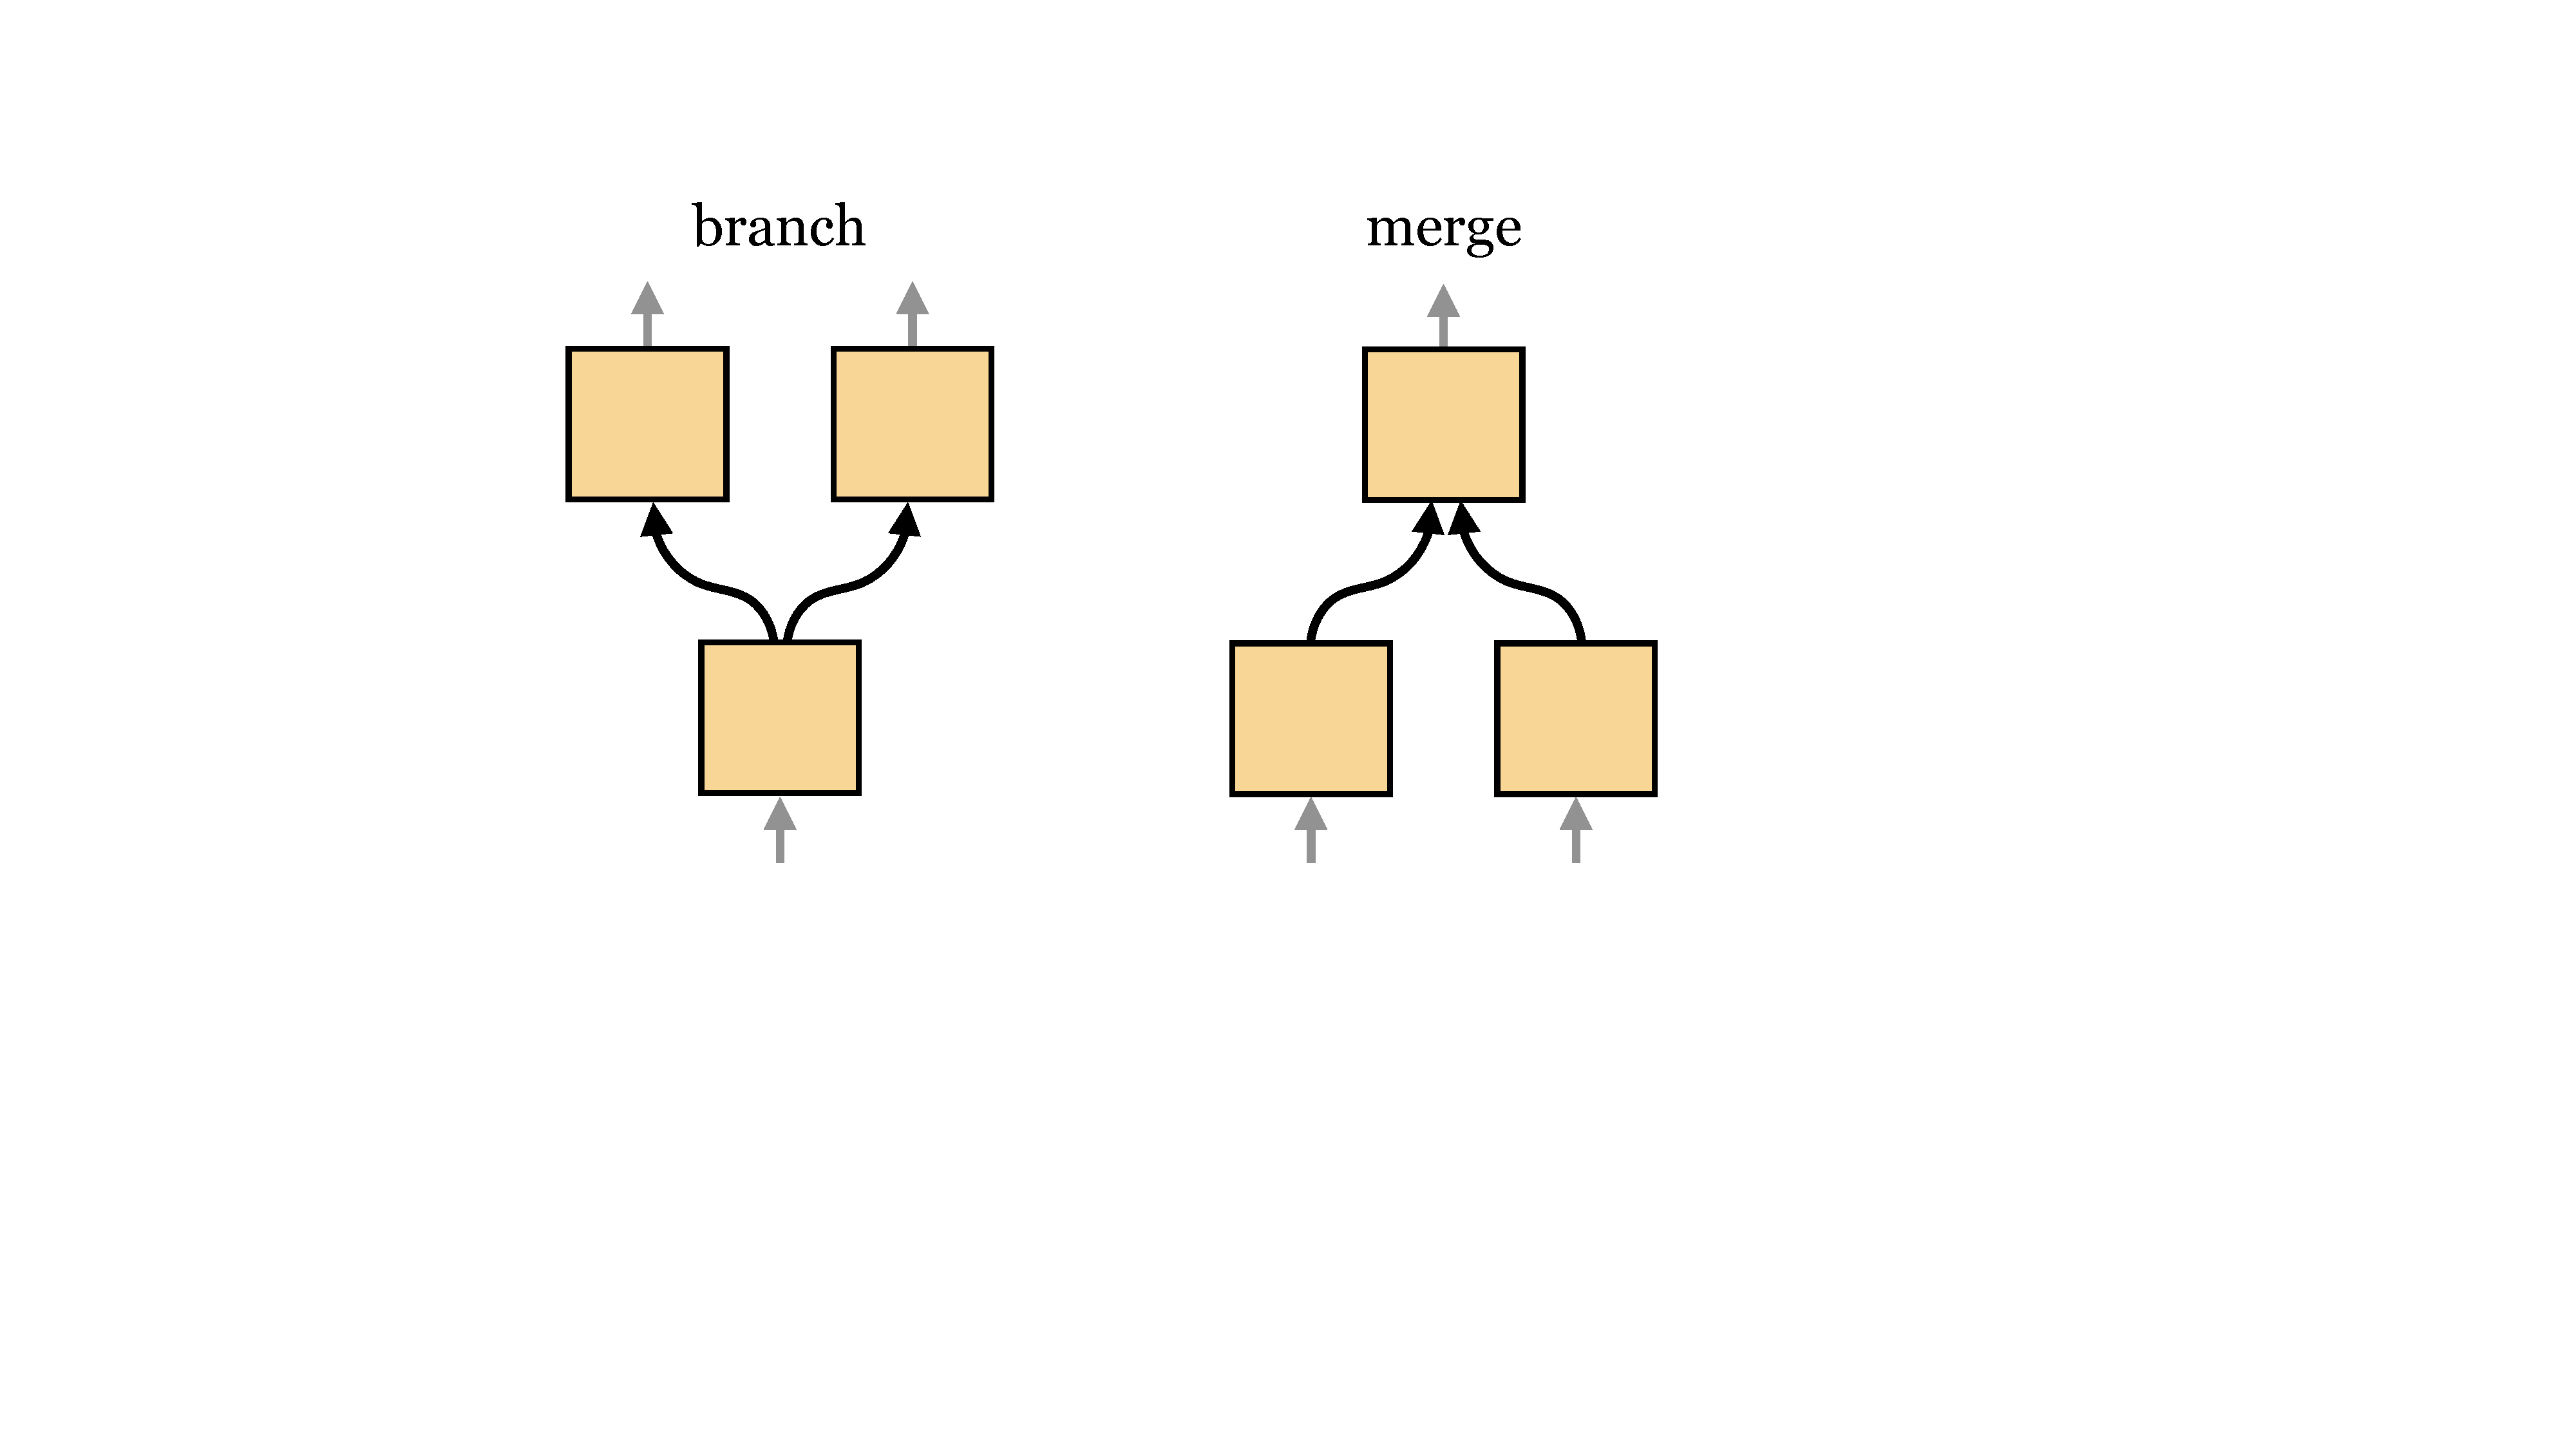
\includegraphics[width=0.42\linewidth]{./figures/backpropagation/branch_merge.pdf}
    \label{fig:backprop_branch_merge}
\end{figure}

\newpage
It turns out to be easier than you might think! A simple way to see how it works is to just define two special new layers, $\texttt{merge}$ and $\texttt{branch}$:
\begin{align}
    \texttt{merge}(\mathbf{x}^a, \mathbf{x}^b, \ldots) &= [\mathbf{x}^a, \mathbf{x}^b, \ldots] \equiv \mathbf{x}^{\texttt{merged}}\\
    \texttt{branch}(\mathbf{x}) &= [\mathbf{x}, \mathbf{x}, \ldots] \equiv [\mathbf{x}^a, \mathbf{x}^b, \ldots]
\end{align}
\marginnote{What if $\mathbf{x}^a$ and $\mathbf{x}^b$ are tensors, or other objects, with different shapes? Can we still concatenate them? The answer is yes. The shape of the data tensor has no impact on the math. We pick the shape just as a notational convenience, e.g., it's natural to think about images as 2D arrays.}[-0.8cm]
$\texttt{merge}$ takes multiple inputs and concatenates them. This results in a new multidimensional variable. The backward pass equation is trivial. To compute the gradient with respect to $\mathbf{x}^{a}$ (and likewise for $\mathbf{x}^b$, $\mathbf{x}^c$, etc), we have
\begin{align}
    \frac{\partial \mathcal{L}}{\partial \mathbf{x}^{a}} &= \frac{\partial \mathcal{L}}{\partial \mathbf{x}^{\texttt{merged}}} \frac{\partial \mathbf{x}^{\texttt{merged}}}{\partial \mathbf{x}^{a}} = \frac{\partial \mathcal{L}}{\partial \mathbf{x}} \frac{\partial \texttt{merge}}{\partial \mathbf{x}^{a}}\\
    &= \frac{\partial \mathcal{L}}{\partial \mathbf{x}^{\texttt{merged}}} [\frac{\partial \mathbf{x}^{1}}{\partial \mathbf{x}^{i}}, \ldots, \frac{\partial \mathbf{x}^{i}}{\partial \mathbf{x}^{i}}, \ldots, \frac{\partial \mathbf{x}^{N}}{\partial \mathbf{x}^{i}}]^T\\
    &= \frac{\partial \mathcal{L}}{\partial \mathbf{x}^{\texttt{merged}}} [0, \ldots, 1, \ldots, 0]^T
\end{align}
That is, we just pick out the i-th block of the $\frac{\partial \mathcal{L}}{\partial \mathbf{x}^{\texttt{merged}}}$ Jacobian matrix. There is really nothing new here. We already defined backprop for multidimensional variables above, and $\texttt{merge}$ is just an explicit way of constructing multidimensional variables.

%We already defined backprop for multidimensional inputs, and nothing is different here. The gradients propagated backwards are $\frac{\partial \mathcal{L}}{\partial \mathbf{x}^{\prime}}$.

\texttt{branch} is only slightly more complicated. In branching, we send copies of the same output to multiple downstream nodes. Therefore, we have multiple gradients coming back to the $\texttt{branch}$ module, each from different downstream paths. So the inputs to this module on the backward pass are $\frac{\partial \mathcal{L}}{\partial \mathbf{x}^{a}}, \frac{\partial \mathcal{L}}{\partial \mathbf{x}^{b}}, \ldots$, which we can write as the Jacobian matrix $\frac{\partial \mathcal{L}}{\partial [\mathbf{x}^a, \mathbf{x}^b, \ldots]} = [\frac{\partial \mathcal{L}}{\partial \mathbf{x}^{a}}, \frac{\partial \mathcal{L}}{\partial \mathbf{x}^{b}}, \ldots]$.  Let's compute the backwards pass output:
\begin{align}
    \frac{\partial \mathcal{L}}{\partial \mathbf{x}} &= \frac{\partial \mathcal{L}}{\partial [\mathbf{x}^a, \mathbf{x}^b, \ldots]} \frac{\partial [\mathbf{x}^a, \mathbf{x}^b, \ldots]}{\partial \mathbf{x}} = \frac{\partial \mathcal{L}}{\partial [\mathbf{x}^a, \mathbf{x}^b, \ldots]} \frac{\partial \texttt{branch}}{\partial \mathbf{x}}\\
    &= [\frac{\partial \mathcal{L}}{\partial \mathbf{x}^{a}}, \frac{\partial \mathcal{L}}{\partial \mathbf{x}^{b}}, \ldots][1, 1, \ldots]^T\\
    &= \sum_{i} \frac{\partial \mathcal{L}}{\partial \mathbf{x}^{i}}
\end{align}
So, branching just sums all the gradients passed backwards to it.
%Suppose our output is $\mathbf{x}^{l+1}$. Then, during backprop, we have multiple different versions of $\partial L \partial x$ being propagated back. How should resolve all these different versions? Consider the simple case where we have two output branches. 

Both $\texttt{merge}$ and $\texttt{branch}$ have no parameters, so there is no parameter gradient to define. Thus, we have fully specified the forward and backward behavior of these layers. 

These diagrams summarize the behavior:
\begin{figure}[h]
    \centering
    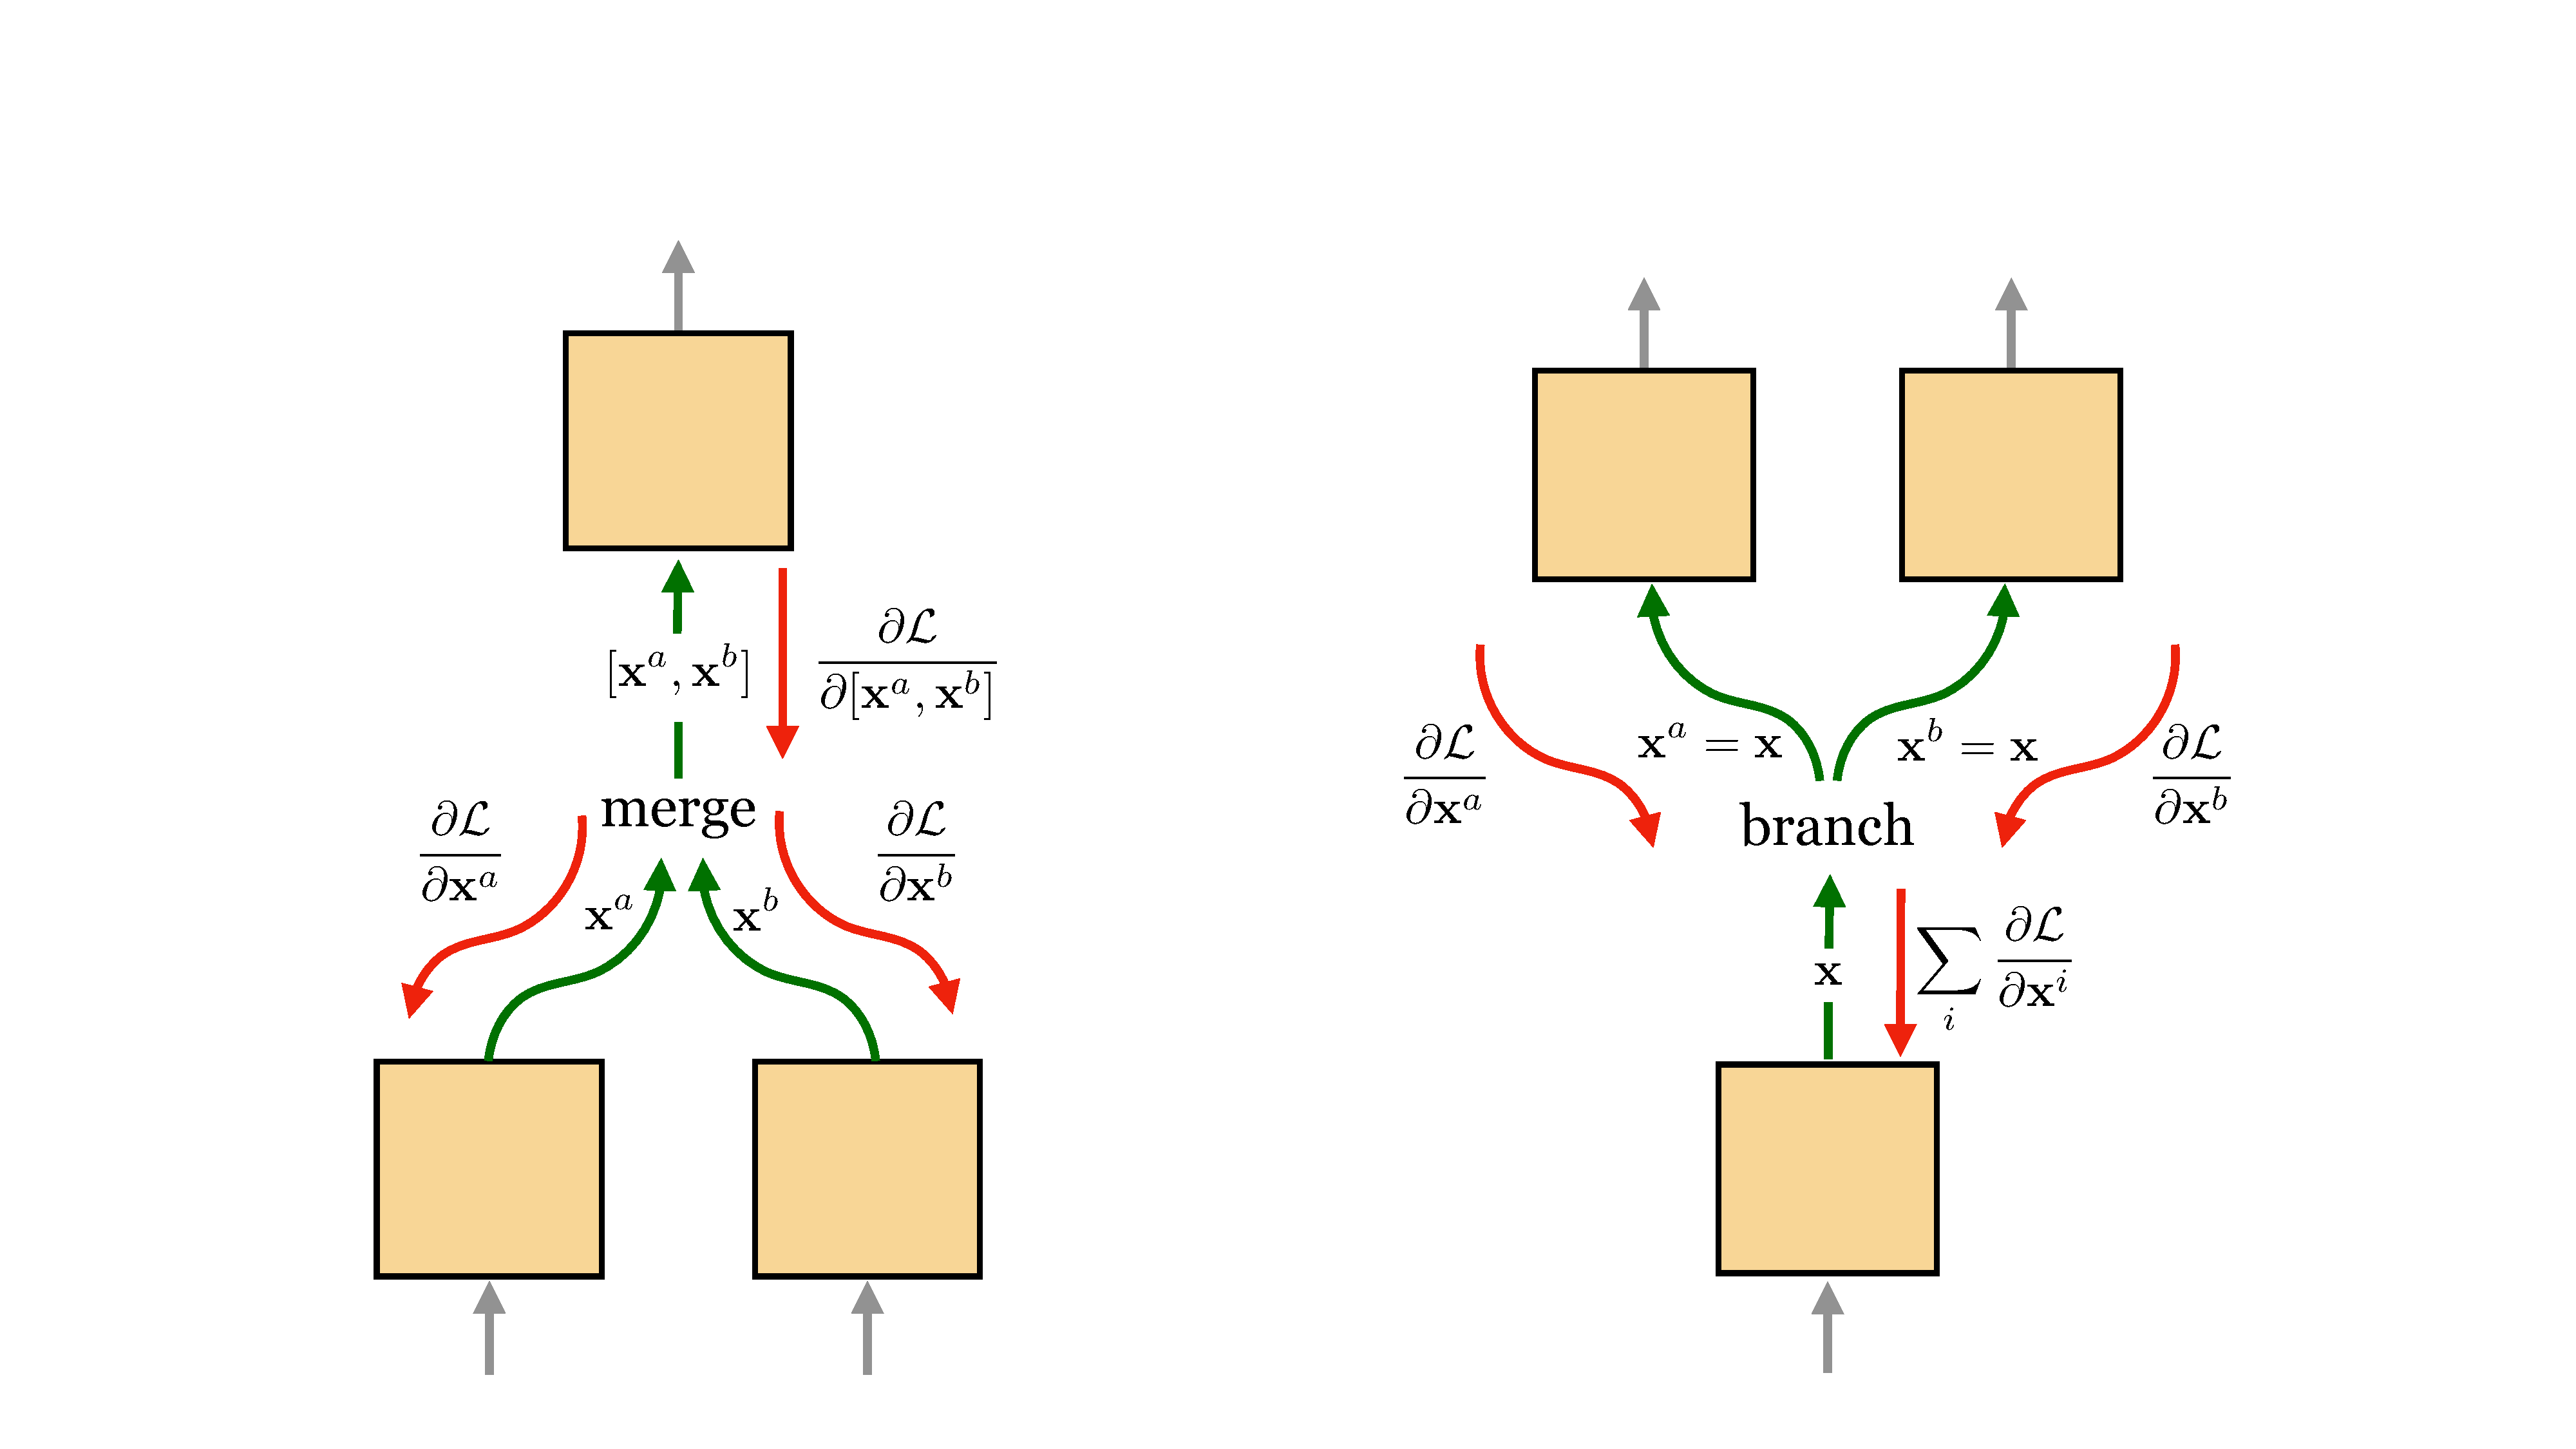
\includegraphics[width=0.75\linewidth]{./figures/backpropagation/branch_merge_gradient_diagrams.pdf}
    \label{fig:backprop_branch_merge_gradient_diagrams}
\end{figure}

\section{Computation graphs}
Now, we can constuct any directed acyclical \textbf{computation graph} (DAG) by simply inserting $\texttt{merge}$ or $\texttt{branch}$ layers wherever we want a node to have multiple inputs, or, respectively, multiple outputs.
\begin{figure}[h]
    \centering
    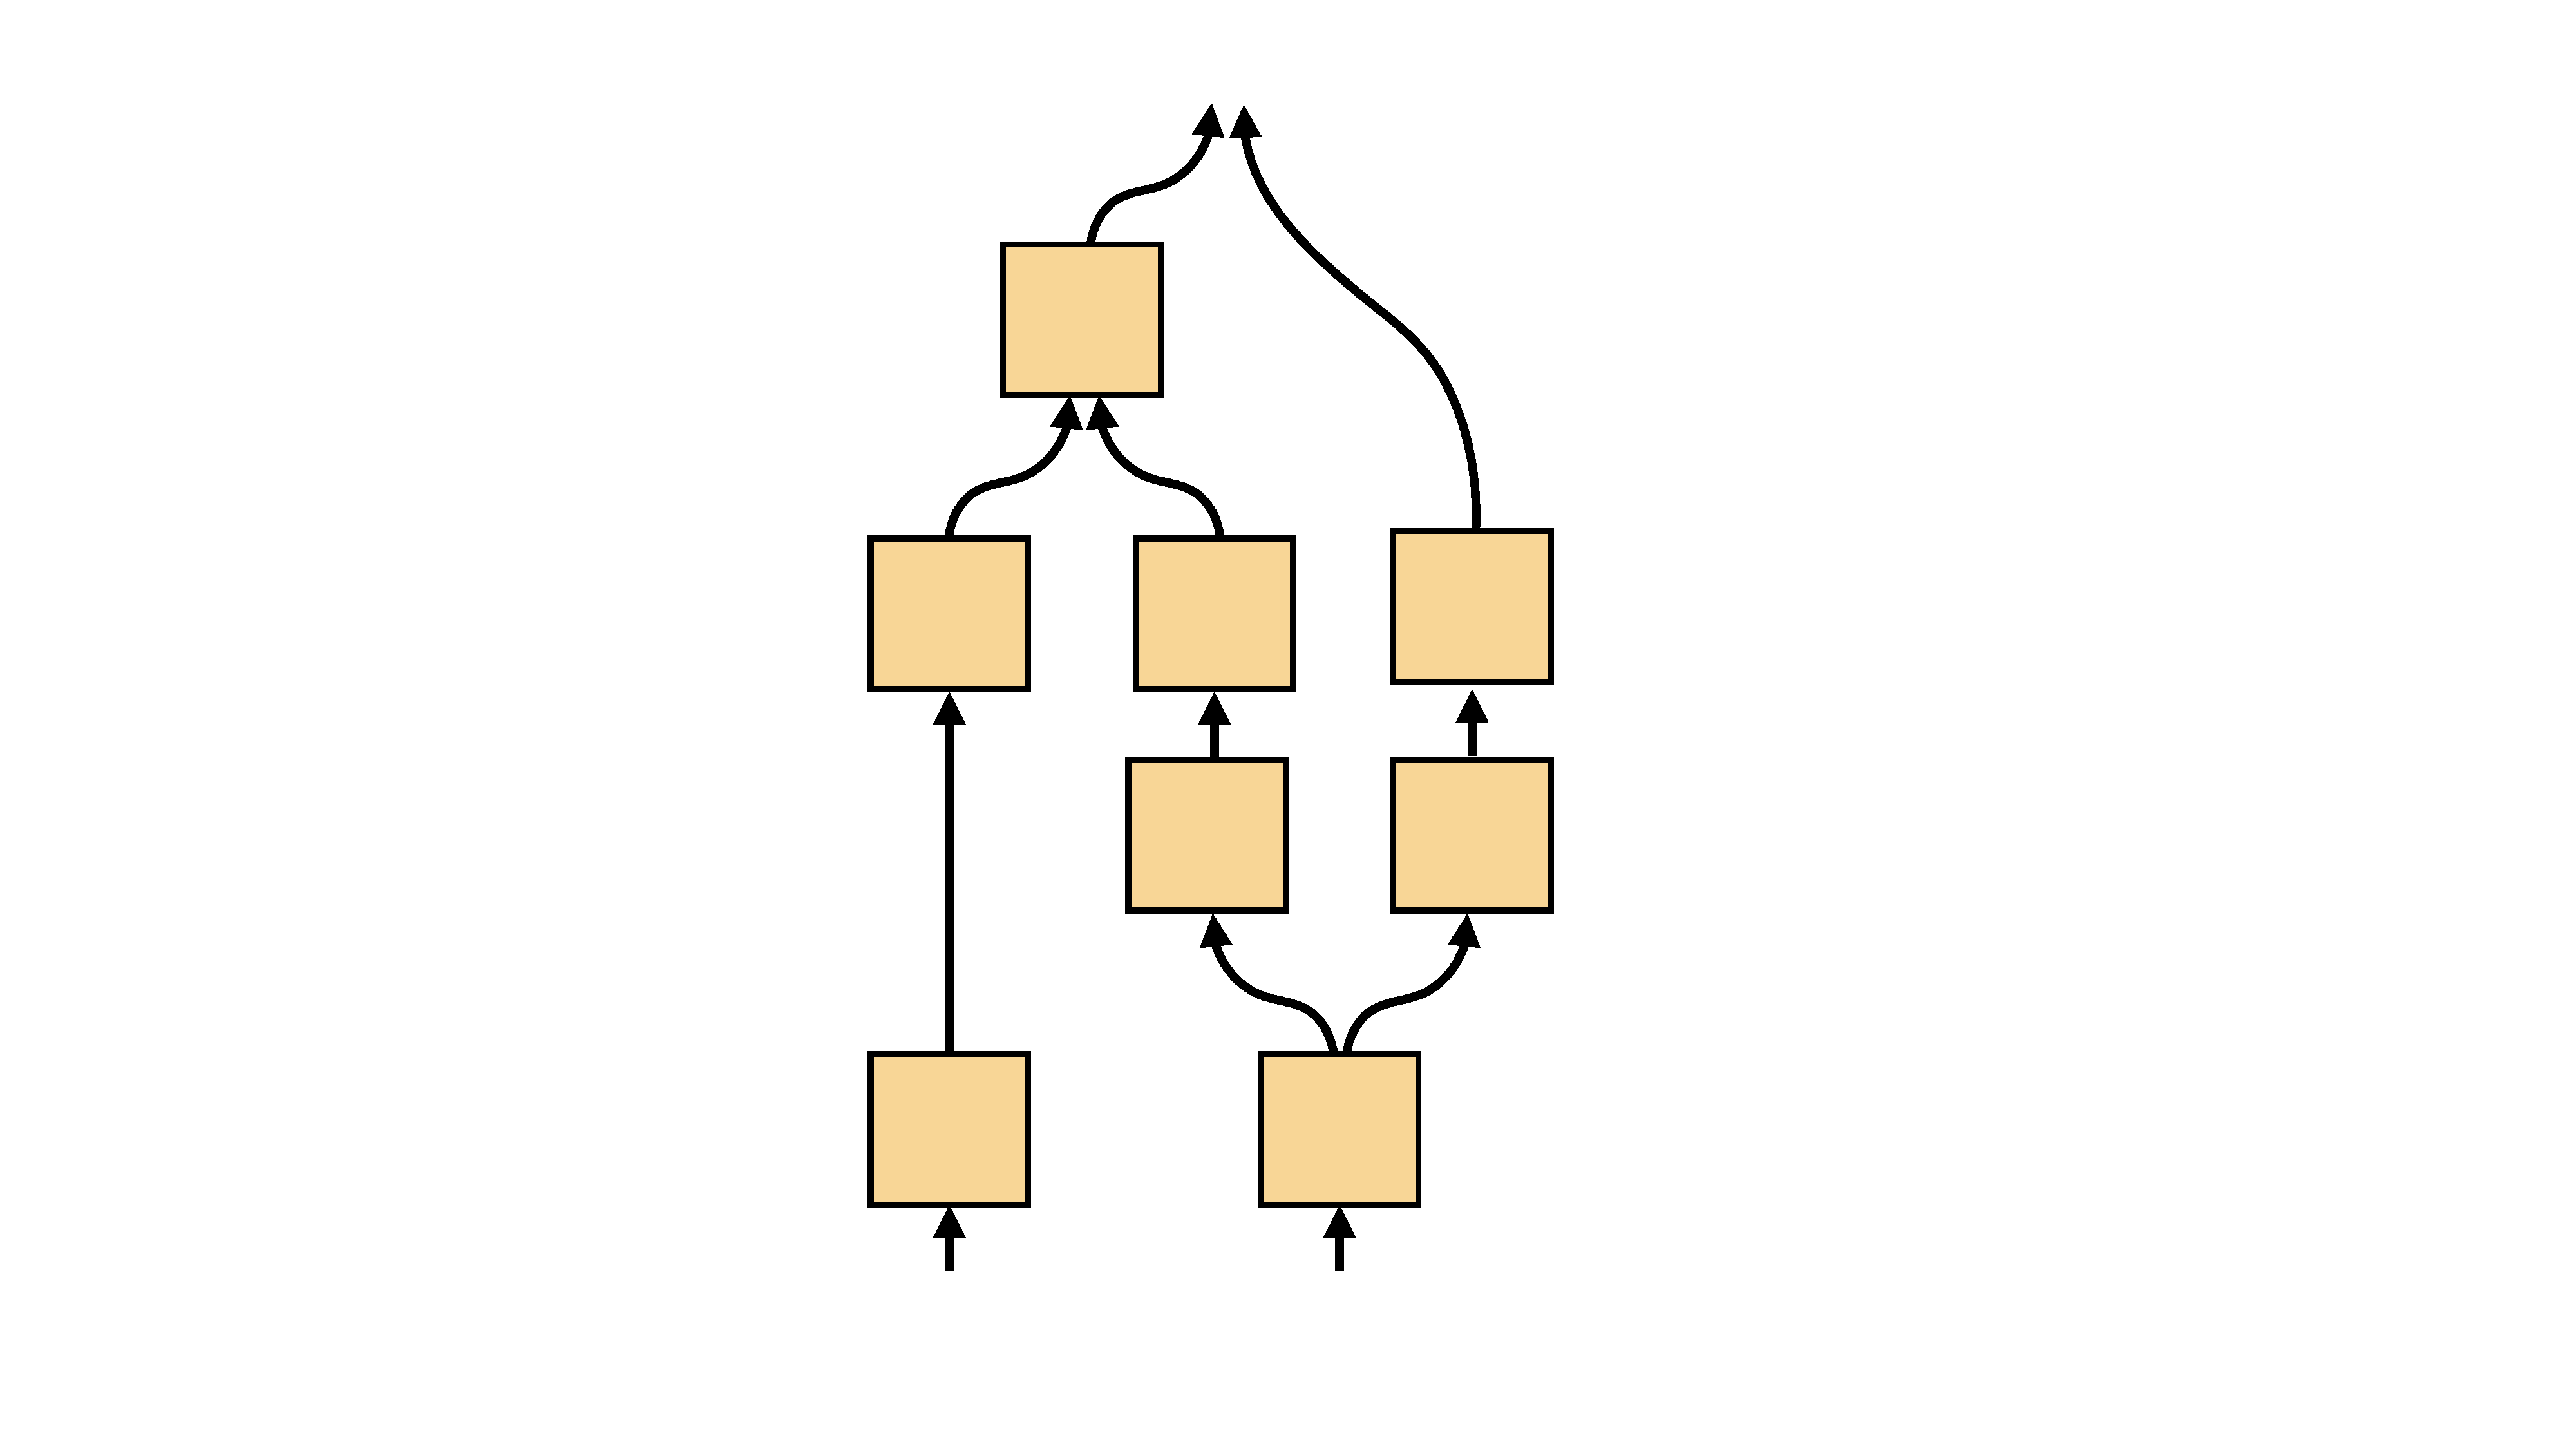
\includegraphics[width=0.16\linewidth]{./figures/backpropagation/DAG.pdf}
    \label{fig:backprop_DAG}
\end{figure}
\marginnote{An example of a DAG computation graph that we can construct, and do backprop through, with the tools defined above.}[1.6cm]

Given a differentiable computation graph, we can optimize any node or edge in the graph w.r.t. any other (scalar) node in the graph. For example, suppose we want to optimize some the value of some cost function (a scalar) indicated as the red node in the computation graph below. Using backprop, we can find and descend the gradient w.r.t. either a mapping at the top of the computation graph (yellow edge), or a w.r.t. some inputs at the bottom (yellow outlined node) or any other edge or node in this graph:
\begin{figure}[h]
    \centering
    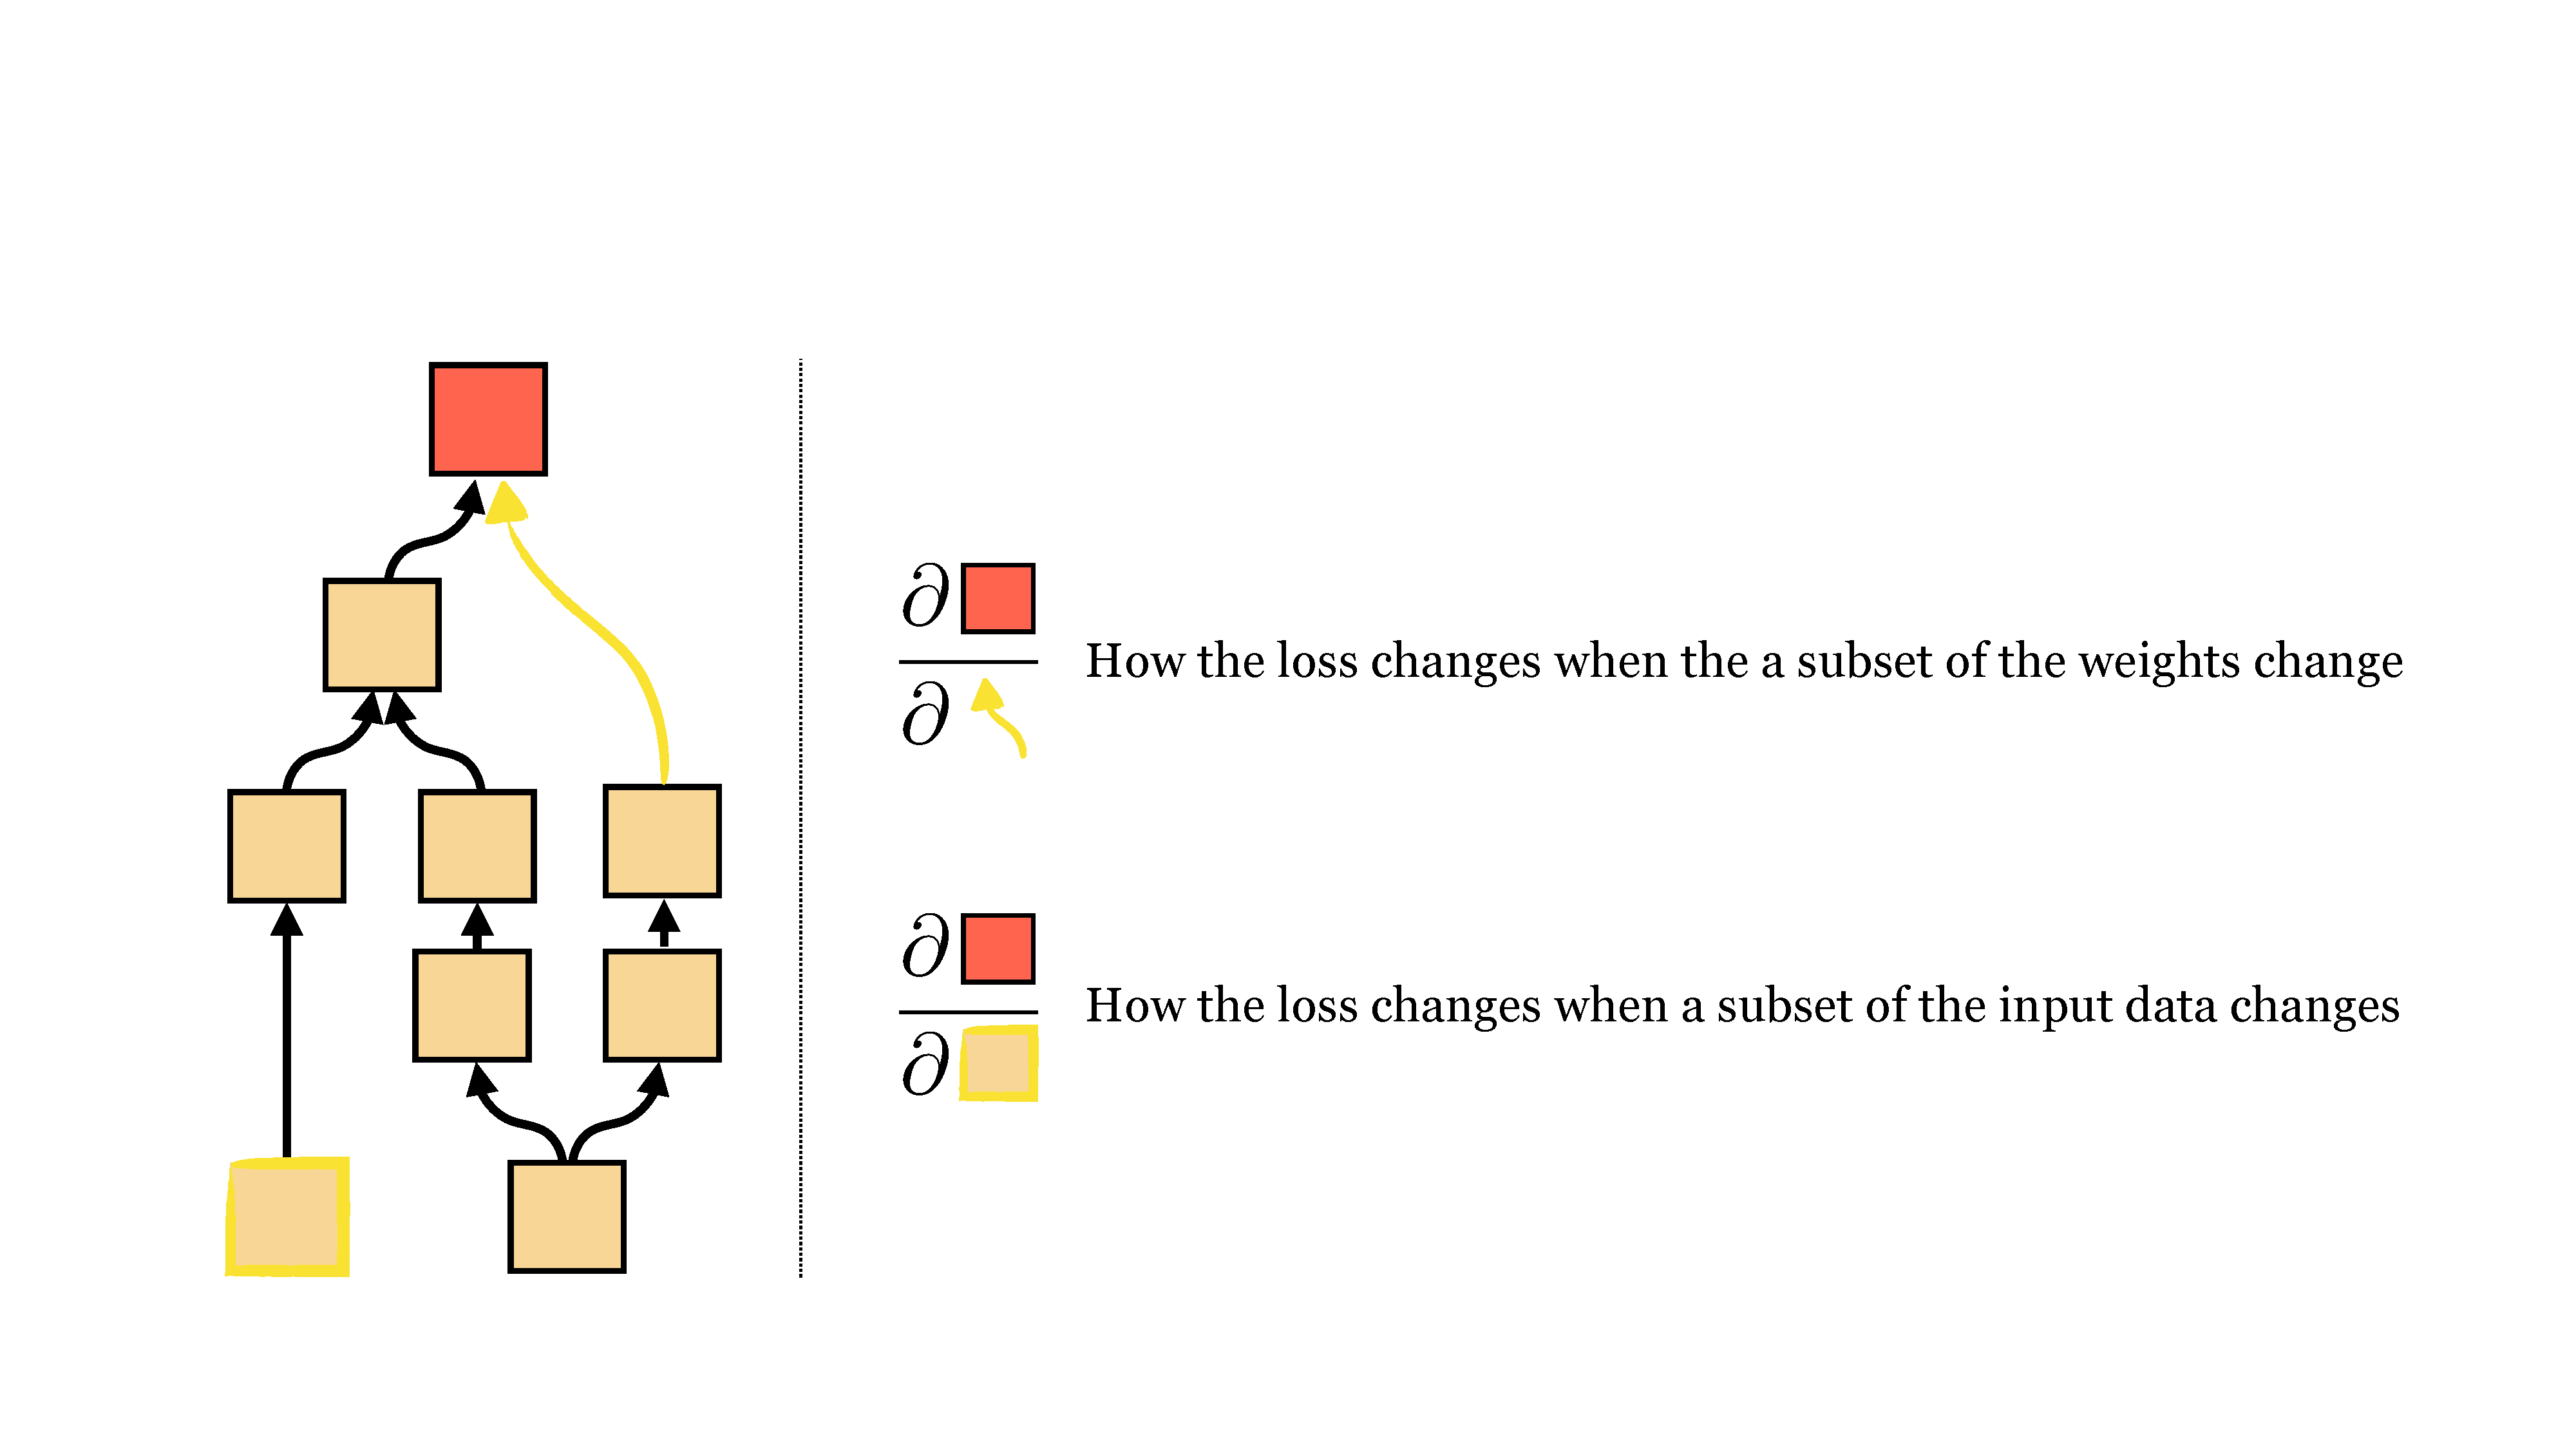
\includegraphics[width=0.9\linewidth]{./figures/backpropagation/computation_graph_opt.pdf}
    \label{fig:computation_graph_opt}
\end{figure}

\section{Differentiable programming}

When $f$ is a layer of a neural network, the algorithm described above is called backpropagation. When $f$ is a generic differentiable function, the algorithm is called reverse mode {\bf automatic differentiation} or {\bf autograd}. The paradigm of programming with compositions of differntiable functions, which are optimized with autograd, is called {\bf differentiable programming}. Using autograd to maximize a learning objective over a hypothesis space of compositions of differentiable functions is a very general purpose learning paradigm, sometimes called {\bf deep learning}.
\marginnote{We use \\{\bf function} $\equiv$ {\bf program} interchangeably.}[-0.8cm]